\documentclass[12pt]{report}
\usepackage[utf8]{inputenc}
\usepackage[T1]{fontenc}
\usepackage{german}
\usepackage{geometry}                % See geometry.pdf to learn the layout options. There are lots.
\usepackage{float}
\geometry{a4paper}                   % ... or a4paper or a5paper or ... 
\usepackage[parfill]{parskip}    % Activate to begin paragraphs with an empty line rather than an indent
\usepackage{xifthen}
\usepackage{xstring}			% to check content of strings in xifthen
\usepackage{graphicx}
\usepackage[usenames,dvipsnames,table]{xcolor}
\usepackage{amssymb}
\usepackage{epstopdf}
\usepackage{hyperref}
\usepackage{fancyhdr}

\definecolor{javared}{rgb}{0.6,0,0} % for strings
\definecolor{javagreen}{rgb}{0.25,0.5,0.35} % comments
\definecolor{javapurple}{rgb}{0.5,0,0.35} % keywords
\definecolor{javadocblue}{rgb}{0.25,0.35,0.75} % javadoc
\definecolor{pblue}{rgb}{0.13,0.13,1}
\definecolor{pgreen}{rgb}{0,0.5,0}
\definecolor{pred}{rgb}{0.9,0,0}
\definecolor{pgrey}{rgb}{0.46,0.45,0.48}

\usepackage{listings}
\lstset{language=Java,
  showspaces=false,
  showtabs=false,
  breaklines=true,
  showstringspaces=false,
  breakatwhitespace=true,
  commentstyle=\color{pgreen},
  keywordstyle=\color{pblue},
  stringstyle=\color{pred},
  basicstyle=\ttfamily,
  moredelim=[il][\textcolor{pgrey}]{\$\$},
  moredelim=[is][\textcolor{pgrey}]{\%\%}{\%\%}
}

\lstdefinelanguage{JavaScript}{
  keywords={typeof, new, true, false, catch, function, return, null, catch, switch, var, if, in, while, do, else, case, break},
  keywordstyle=\color{blue}\bfseries,
  ndkeywords={class, export, boolean, throw, implements, import, this},
  ndkeywordstyle=\color{darkgray}\bfseries,
  identifierstyle=\color{black},
  sensitive=false,
  comment=[l]{//},
  morecomment=[s]{/*}{*/},
  commentstyle=\color{purple}\ttfamily,
  stringstyle=\color{red}\ttfamily,
  morestring=[b]',
  morestring=[b]"
}

\lstset{
   language=JavaScript,
   extendedchars=true,
   basicstyle=\footnotesize\ttfamily,
   showstringspaces=false,
   showspaces=false,
   numbers=left,
   numberstyle=\footnotesize,
   numbersep=9pt,
   tabsize=2,
   breaklines=true,
   showtabs=false,
   captionpos=b
}


\IfStrEq*{\languagename}{english}
	{
		\newcommand{\dalabel}{Diploma Thesis}
		\newcommand{\submittedlabel}{Submitted by}
		\newcommand{\datelabel}{Date}
		\newcommand{\supervisorlabel}{Supervisor}
		\newcommand{\projectpartnerlabel}{Project Partner}
	}
	{
		\newcommand{\dalabel}{Diplomarbeit}
		\newcommand{\submittedlabel}{Eingereicht von}
		\newcommand{\datelabel}{Datum}
		\newcommand{\supervisorlabel}{Betreuer}
		\newcommand{\projectpartnerlabel}{Projektpartner}
	}
 % This file should not really be touched
\newcommand{\titleofthesis}{HomeDS}
\newcommand{\department}{Informatik} % Replace by your department

\newcommand{\firstauthor}{Andrej Sakal}
\newcommand{\firstauthorclass}{5CHIF}
\newcommand{\secondauthor}{Felix Hofmann}
\newcommand{\secondauthorclass}{5CHIF}

\newcommand{\duedateen}{April 4, 2018} % due date in english format
\newcommand{\duedatede}{4. April 2018} % due date in german format
\newcommand{\supervisor}{Thomas Stütz}

 % Set basic data (author, title, etc.) of your thesis
\begin{document}
\rhead{
\includegraphics[scale=.9]{images/Logo.png}}
\cfoot{}
\begin{titlepage}
\thispagestyle{fancy}

\begin{center}

\vspace*{8em}

{\LARGE \dalabel}

\vspace{2em}

{\large Höhere Technische Bundeslehranstalt Leonding \\[.5em]
Abteilung für \department}

%\vspace{8em}
\vspace*{\fill}

{\Huge \titleofthesis}
\end{center}

%\vspace{8em}
\vspace*{\fill}

\begin{tabular}{ll}
\ifthenelse{\isundefined{\firstauthor}}{}{\submittedlabel: & {\bf \firstauthor, \firstauthorclass}}
\ifthenelse{\isundefined{\secondauthor}}{}{ \\[.5em] & {\bf \secondauthor, \secondauthorclass}}
\ifthenelse{\isundefined{\thirdauthor}}{}{ \\[.5em] & {\bf \thirdauthor, \thirdauthorclass}}
\ifthenelse{\isundefined{\fourthauthor}}{}{ \\[.5em] & {\bf \fourthauthor, \fourthauthorclass}}
 \\[.5em]
\datelabel: & {\bf \duedateen} \\[.5em]

\supervisorlabel: & {\bf \supervisor} \\[.5em]

\ifthenelse{\isundefined{\projectpartner}}{}{\projectpartnerlabel: & {\bf \projectpartner}}
\end{tabular}
\end{titlepage}
 % Should not be necessary to touch this file
\section*{Declaration of Academic Honesty}
Hereby, I declare that I have composed the presented paper independently on my own and without any other resources than the ones indicated. All thoughts taken directly or indirectly from external sources are properly denoted as such.

This paper has neither been previously submitted to another authority nor has it been published yet. \\[1em]
Leonding, \duedateen \\[5em]
\vspace{1.5cm}
\begin{center}
\begin{tabularx}{\textwidth}[b]{p{5cm} X p{5cm}} \cline{1-1} \cline{3-3}
Andrej Sakal & & Felix Hofmann
\end{tabularx}
\end{center}

\begin{otherlanguage}{german}
\section*{Eidesstattliche Erklärung}
Hiermit erkläre ich an Eides statt, dass ich die vorgelegte Diplomarbeit selbstständig und ohne Benutzung anderer als der angegebenen Hilfsmittel angefertigt habe. Gedanken, die aus fremden Quellen direkt oder indirekt übernommen wurden, sind als solche gekennzeichnet.

Die Arbeit wurde bisher in gleicher oder ähnlicher Weise keiner anderen Prüfungsbehörde vorgelegt und auch noch nicht veröffentlicht. \\[1em]
Leonding, am \duedatede \\[5em]
\begin{center}
\begin{tabularx}{\textwidth}[b]{p{5cm} X p{5cm}} \cline{1-1} \cline{3-3}
Andrej Sakal & & Felix Hofmann
\end{tabularx}
\end{center}
\end{otherlanguage}


\begin{otherlanguage}{english}
\begin{abstract}
The HomeDS is a compact digital signage system that is tailored to the requirements. This allows the user to access Signage System features without having to read the signage system manual.

The result of this work is a web interface and an Android application for mobile devices. These should fulfill the functional scope described in the task.
\end{otherlanguage}


\begin{otherlanguage}{german}
\begin{abstract}
Beim HomeDS handelt es sich um ein kompaktes Digital Signage System, das auf die ausgewählten Anforderungen zugeschnitten ist. Dadurch wird ermöglicht, dass der Benutzer auf Funktionen des Signage System zugreifen kann ohne sich in das Handbuch eines Signage System einlesen zu müssen. 

Das Ergebnis dieser Arbeit ist eine Weboberfläche und eine Android Applikation für mobile Endgeräte. Diese sollen den Funktionsumfang, welcher in der Aufgabenstellung beschrieben ist, erfüllen.
\end{otherlanguage}

\newpage

% Danksagung
\section*{Danksagung}
\begin{normalsize}
An dieser Stelle möchten wir uns sehr herzlich bei der HTBLA Leonding für die kompetente Betreuung und Unterstützung der letzten Jahre bedanken. Insbesondere sind wir auch Prof. Mag. Dr. Stütz zu tiefstem Dank verpflichtet, welcher uns während des Projektes tatkräftig zur Seite stand und jederzeit für Fragen erreichbar war.
Natürlich möchten wir auch unseren Eltern und Bezugspersonen einen herzlichen Dank aussprechen, welche in den letzten Jahren stets ein offenes Ohr für unsere Probleme hatten und uns auch in schwierigeren Zeiten ein Ansporn waren.
\end{normalsize}\\
\newpage

 % Declaration of Academic Honesty, Abstracts, Acknowledgments, 

\tableofcontents

\chapter{Einleitung}
\section{Ausgangssituation}
Die HTL-Leonding besitzt schon einige Multimedia Systeme verstreut im ganzen Schulgeb�ude um Projekte, aktuelle News und �nderungen im Unterrichtsablauf anzuzeigen. Doch ein gro�er Schwachpunkt dieser Multimedia Systeme ist, dass der Prozess vom erstellen der Anzeige bis zum zuordnen welcher Bildschirm, welche Information anzeigen soll sehr kompliziert, und m�hselig ist. Sodass oftmals neue Informationen erst Versp�tet oder gar nicht angezeigt wird. 

\section{Ziele}
Ziel ist es, dass es der Schulverwaltung m�glich ist Informationen, Warnungen oder Ank�ndigungen m�glichst schnell �berall in der Schule anzuzeigen. Die verschiedenen Multimediasysteme sollen einheitlich gesteuert und verwaltet werden k�nnen um schnell alle Anzeigen beliebig zu ver�ndern. So ist es auch ein Teilziel festzustellen ob es m�glich die derzeitig verwendeten Anzeigesysteme durch den XIBO Server zu ersetzen.

\section{Problemstellung}
Momentan wird um eine Anzeige zu �ndern sehr viel Aufwand betrieben, zum Beispiel wird eine neue Pr�sentation erstellt in Form von Folien oder ein Video zusammengeschnitten Beispiel daf�r ist die Anzeige im Eingangsbereich der Schule. Diese Vorgehensweise ist zeitaufwendig und werden �nderungen vorgenommen, kann man die alte Pr�sentation oder das Video meistens verwerfen.

\section{Overview}
Details of the diploma thesis have to be aligned between student and supervisor. This should be a basic structure to facilitate the first steps when students start to write their theses.

Never forget to add some illustrative images. Images must not be messed up with your normal text. They are encapsulated in floating bodies and referenced in your text. An example can be seen in figure~\ref{fig:sample}. As you can see, figures are placed by default on top of the page nearby the place where they are referenced the first time. Furthermore you can see that a list of figures is maintained automatically which can be included easily by typing the command \verb1\listoffigures1 into your document.

\begin{figure}
\begin{center}
	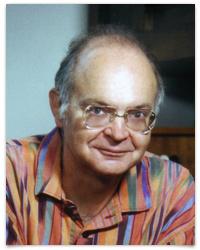
\includegraphics[scale=.5]{images/don_knuth.jpg}
\end{center}
	\caption{Don Knuth, the inventor of \TeX}
	\label{fig:sample}
\end{figure}

\section{Basic Terminology}
As usual the very basic terminology is briefly explained here. Most probably the explanations here only scratch a surface level. More detailed explanations of terminology goes into chapter~\ref{cha:theoretical-background}.

\section{Related Work and Projects}
Here a survey of other work in and around the area of the thesis is given. The reader shall see that the authors of the thesis know their field well and understand the developments there. Furthermore here is a good place to show what relevance the thesis in its field has.

\section{Structure of the Thesis}
%dsflkjas flaksjfl asdfj as lfjldsajflaksdjf sa dfjlasdkfj sadlfjasdklf als dfj l dfsdfsdfn chapter~\ref{cha:used-technologies} (\nameref{cha:used-technologies}) on page~\pageref{cha:used-technologies} we describe the used technologies.
Finally the reader is given a brief description what (s)he can expect in the thesis. Each chapter is introduced with a paragraph roughly describing its content.
\chapter{Digital Signage & XIBO}
\section{Was ist Digital Signage?}\label{sec:digitalsignage}
Digital Signage, in Deutsch Digitales Schild, hat grundsätzlich die Aufgabe Inhalte die meist auf Plakaten oder Schildern angezeigt werden auf Bildschirmen anzuzeigen. Mithilfe von Digital Signage Systemen, soll das zeit- oder interaktionsgesteuerte Ändern von Inhalten auf den Bildschirmen einfach und übersichtlich gehalten werden siehe Abbildung \ref{img:digitalsignagehtlleonding}. Weiteres bietet Digital Signage ein breites Spektrum an Anwendungsbereichen. Digital Signage ist vor allem im Marketing Bereich ein sehr beliebtes Mittel, um ein neues Produkt oder eine Neuheit zu präsentieren. 

https://de.wikipedia.org/wiki/Digital_Signage#Anwendungsbeispiele:_2017.


\begin{figure}[H]
\centering
\includegraphics[width=1\textwidth]{images/02_XiboGrundlagen/Videowall.JPG}
\caption{Digital Signage in der HTL Leonding}
\label{img:digitalsignagehtlleonding}
\end{figure}

\section{Digital Signage Anwendungen}\label{sec:anwendungedigitalsignage}
Digital Signage hat keine Grenzen und kann vielfältig eingesetzt werden. Viele Konzerne nutzen Digital Signage für Marketing Zwecke, Produkte zu präsentieren oder oft auch nur als Lockmittel.

\section{Was ist XIBO?}\label{sec:xibo}
Das XIBO ist ein Open Source Digital Signage System entwickelt von der Spring Signage LTD. Das XIBO-System besteht aus vielen verschiedenen Komponenten. Das XIBO Paket besteht aus einem klassischen Server-Client Konstrukt. Der Server besteht aus drei Komponenten: das Content Managment System welches mithilfe von ZeroMq bei Änderung der Inhalte diese aktualisieren soll, einer Datenbank und einer Weboberfläche, die es dem Benutzer ermöglichen soll das System zu bedienen.

\section{Weboberfläche des XIBO}\label{sec:webpagexibo}
Das Steuerungszentrum des ganzen Signage System ist die Weboberfläche, die ganz einfach über einen Browser unter der Serveraddresse aufgerufen werden kann. Auf der Willkommensseite sind die wichtigsten Funktionen des Signage Servers dargestellt:

\begin{enumerate}
	\item {\em Kalender:} Mit der Kalender Funktion kann eingetragen werden zu welchem Zeitpunkt, welcher Inhalt, auf welchem Bildschirm angezeigt werden soll. Diese Funktion ist einer der wichtigsten und meist verwendeten. In dem Xibo-Kalender werden auch bereits eingetragene Aktivitäten angezeigt.

\begin{figur}
	\centering
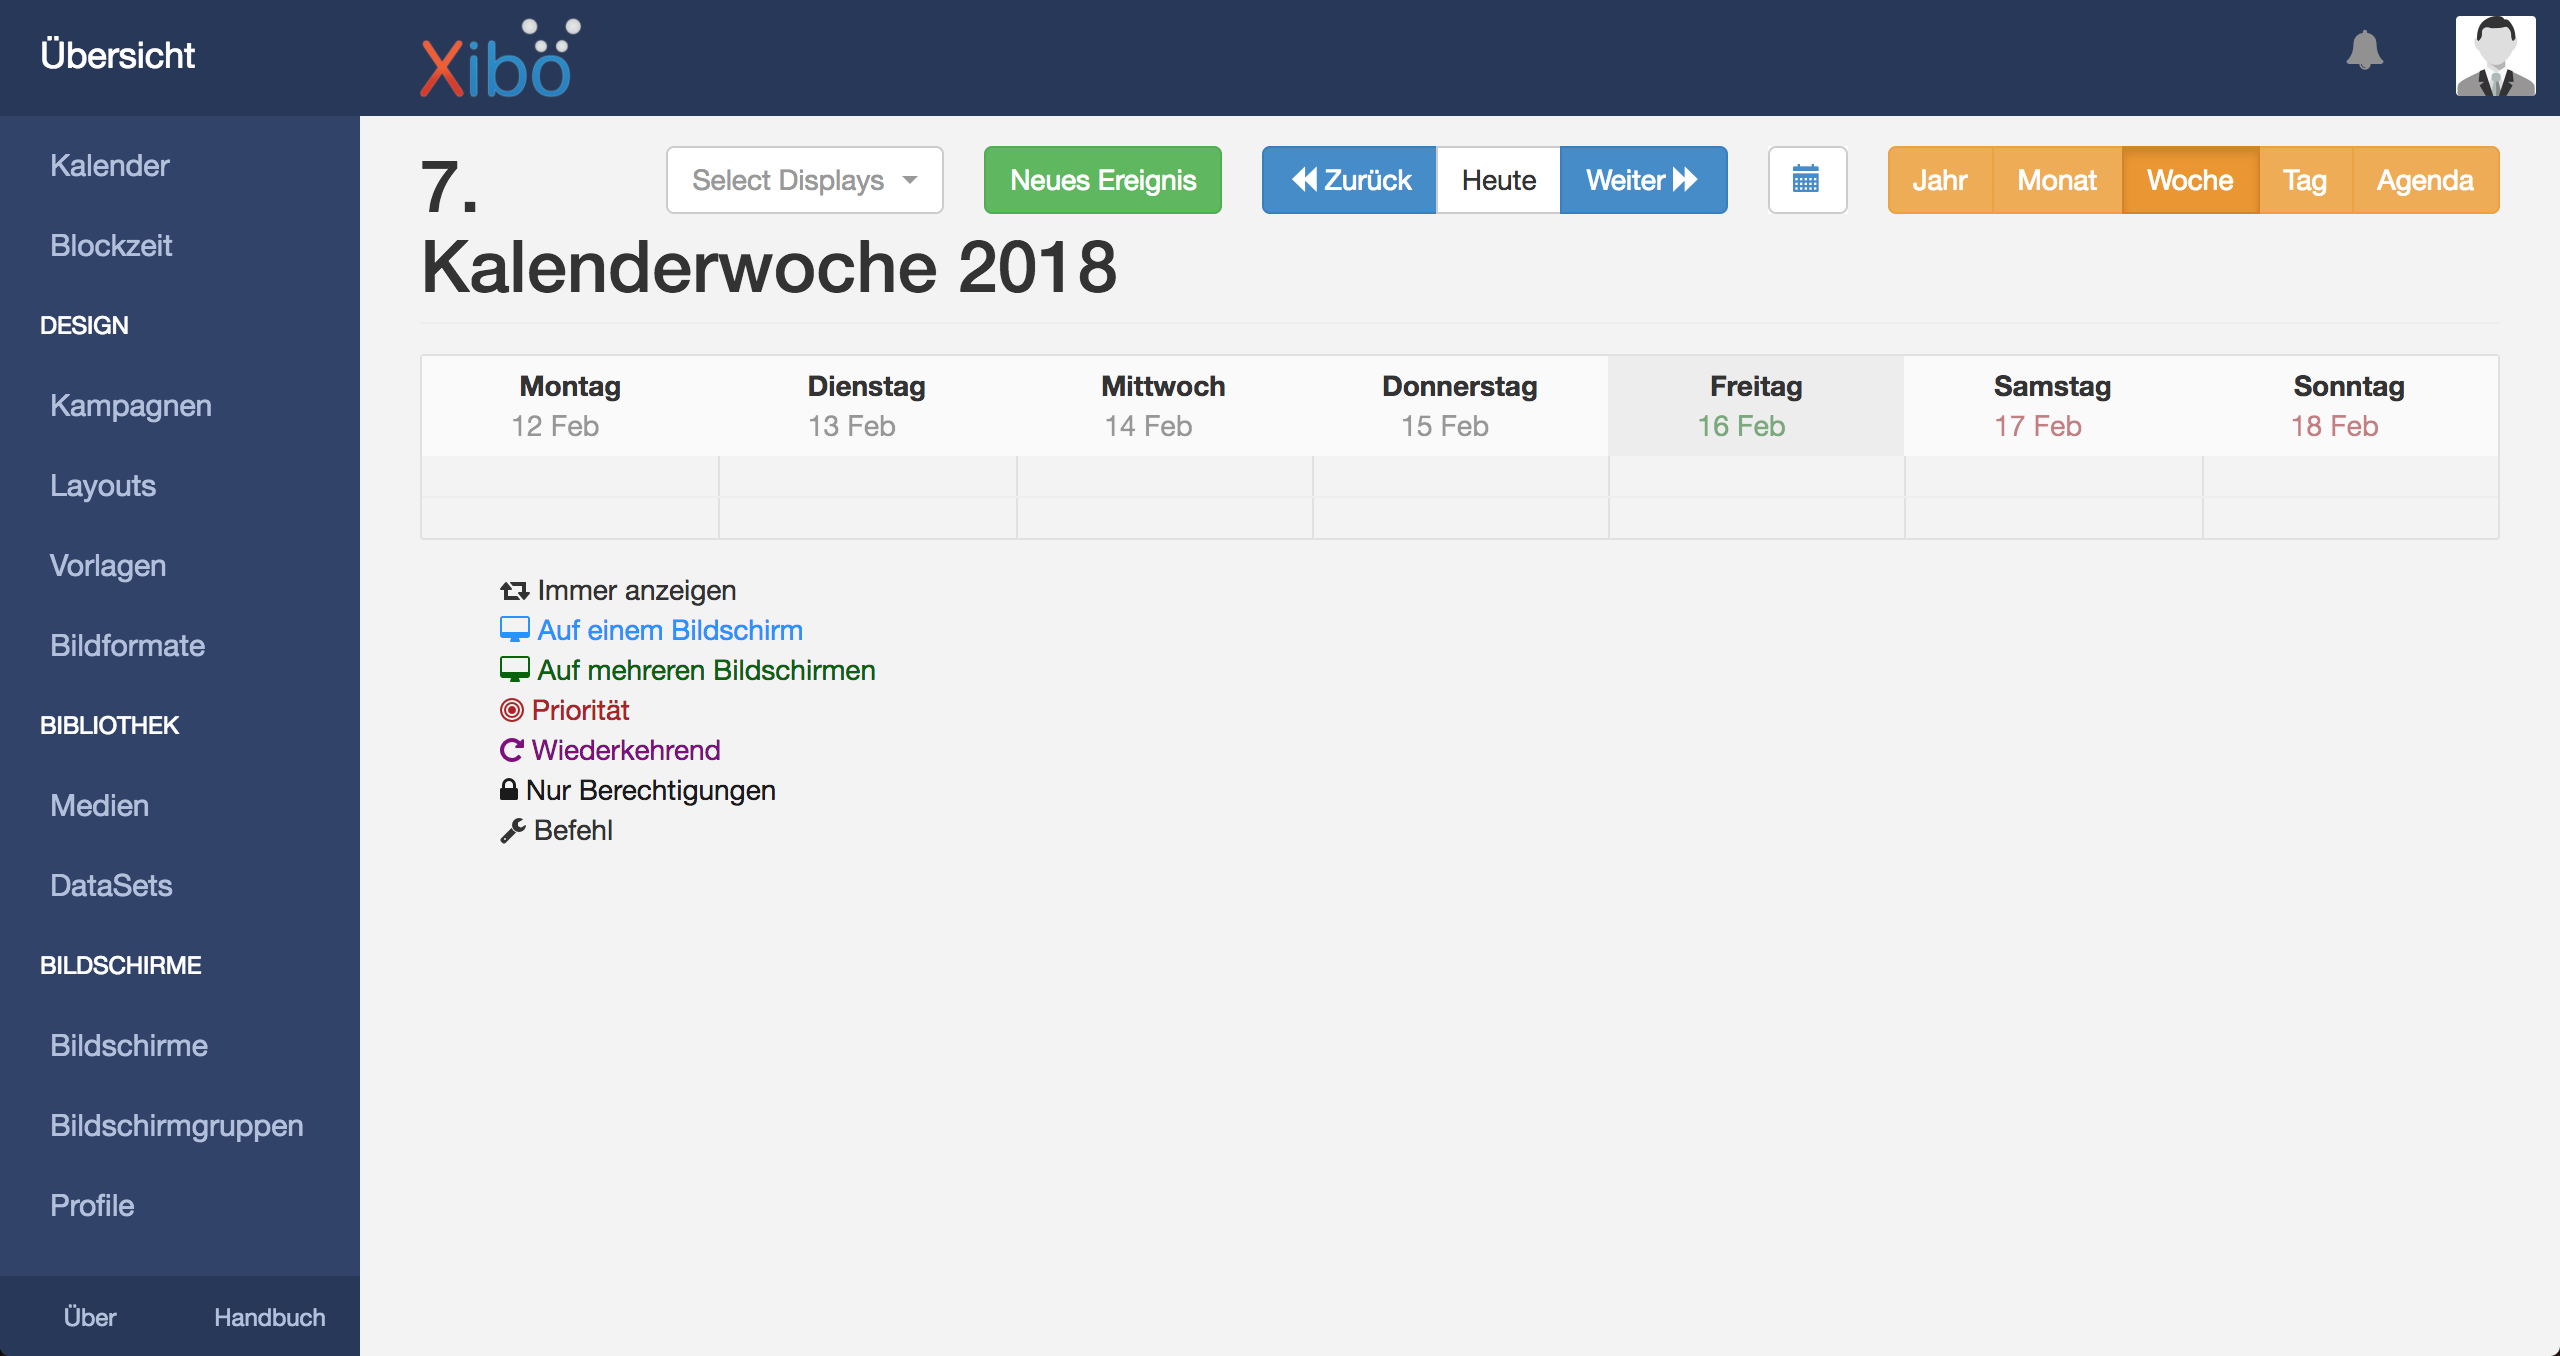
\includegraphics[width=1\textwidth]{images/xibo-basics-calendar}
	\label{img:calendar}
	\caption{XBIO - Kalender}
\end{calendar}	
	
	\item {\em Layouts:} 
	Die Layout-Funktion ist einer der wichtigsten Komponenten des Signage Systems. Es beschäftigt sich mit dem Designen der Inhalte. Auf diese Funktion kommen wir noch einmal zurück.
	
	\item {\em Bibliothek:} 
	Die Bibliothek-Funktion ist zuständig für das Verwalten der Medien. Hier können Sie verschiedene Dateien hochladen.  Diese Medien können dann in Layouts eingebunden und angezeigt werden.
	
	\item {\em Benutzer:} 
	Im Menüpunkt Benutzer können neue Benutzer angelegt und bereits bestehende bearbeitet oder gelöscht werden. Dabei gibt es auch ein Rechte-System. Es können auch Datenmengenbegrenzungen pro Benutzer eingestellt werden.
	
	\item {\em Einstellungen:} 
	Der Menüpunkt Einstellungen gibt dem Nutzer die Möglichkeit, verschiedene Optionen zu wählen. So sind zum Beispiel die richtige Zeitzone, E-Mail Benachrichtigungen, wichtige Einstellungen, die für ein einwandfreies Funktionieren des Xibo-Servers zuständig sind. Aus den Einstellungen ist auch der CMS geheimer Schlüssel zu finden, der für die Authentifizierung der API Zugriffe zuständig ist herauszulesen.
\end{enumerate}

\section{Designen mit XIBO}\label{sec:designexibo}
Beim Designen von einem neuen Layout im XIBO, muss zuerst die Bildschirmauflösung ausgewählt und dem Layout ein passender Name zugewiesen werden, sowie optional auch eine Beschreibung. 

\textbf{Layout Maske}

\begin{calendar}
	\centering
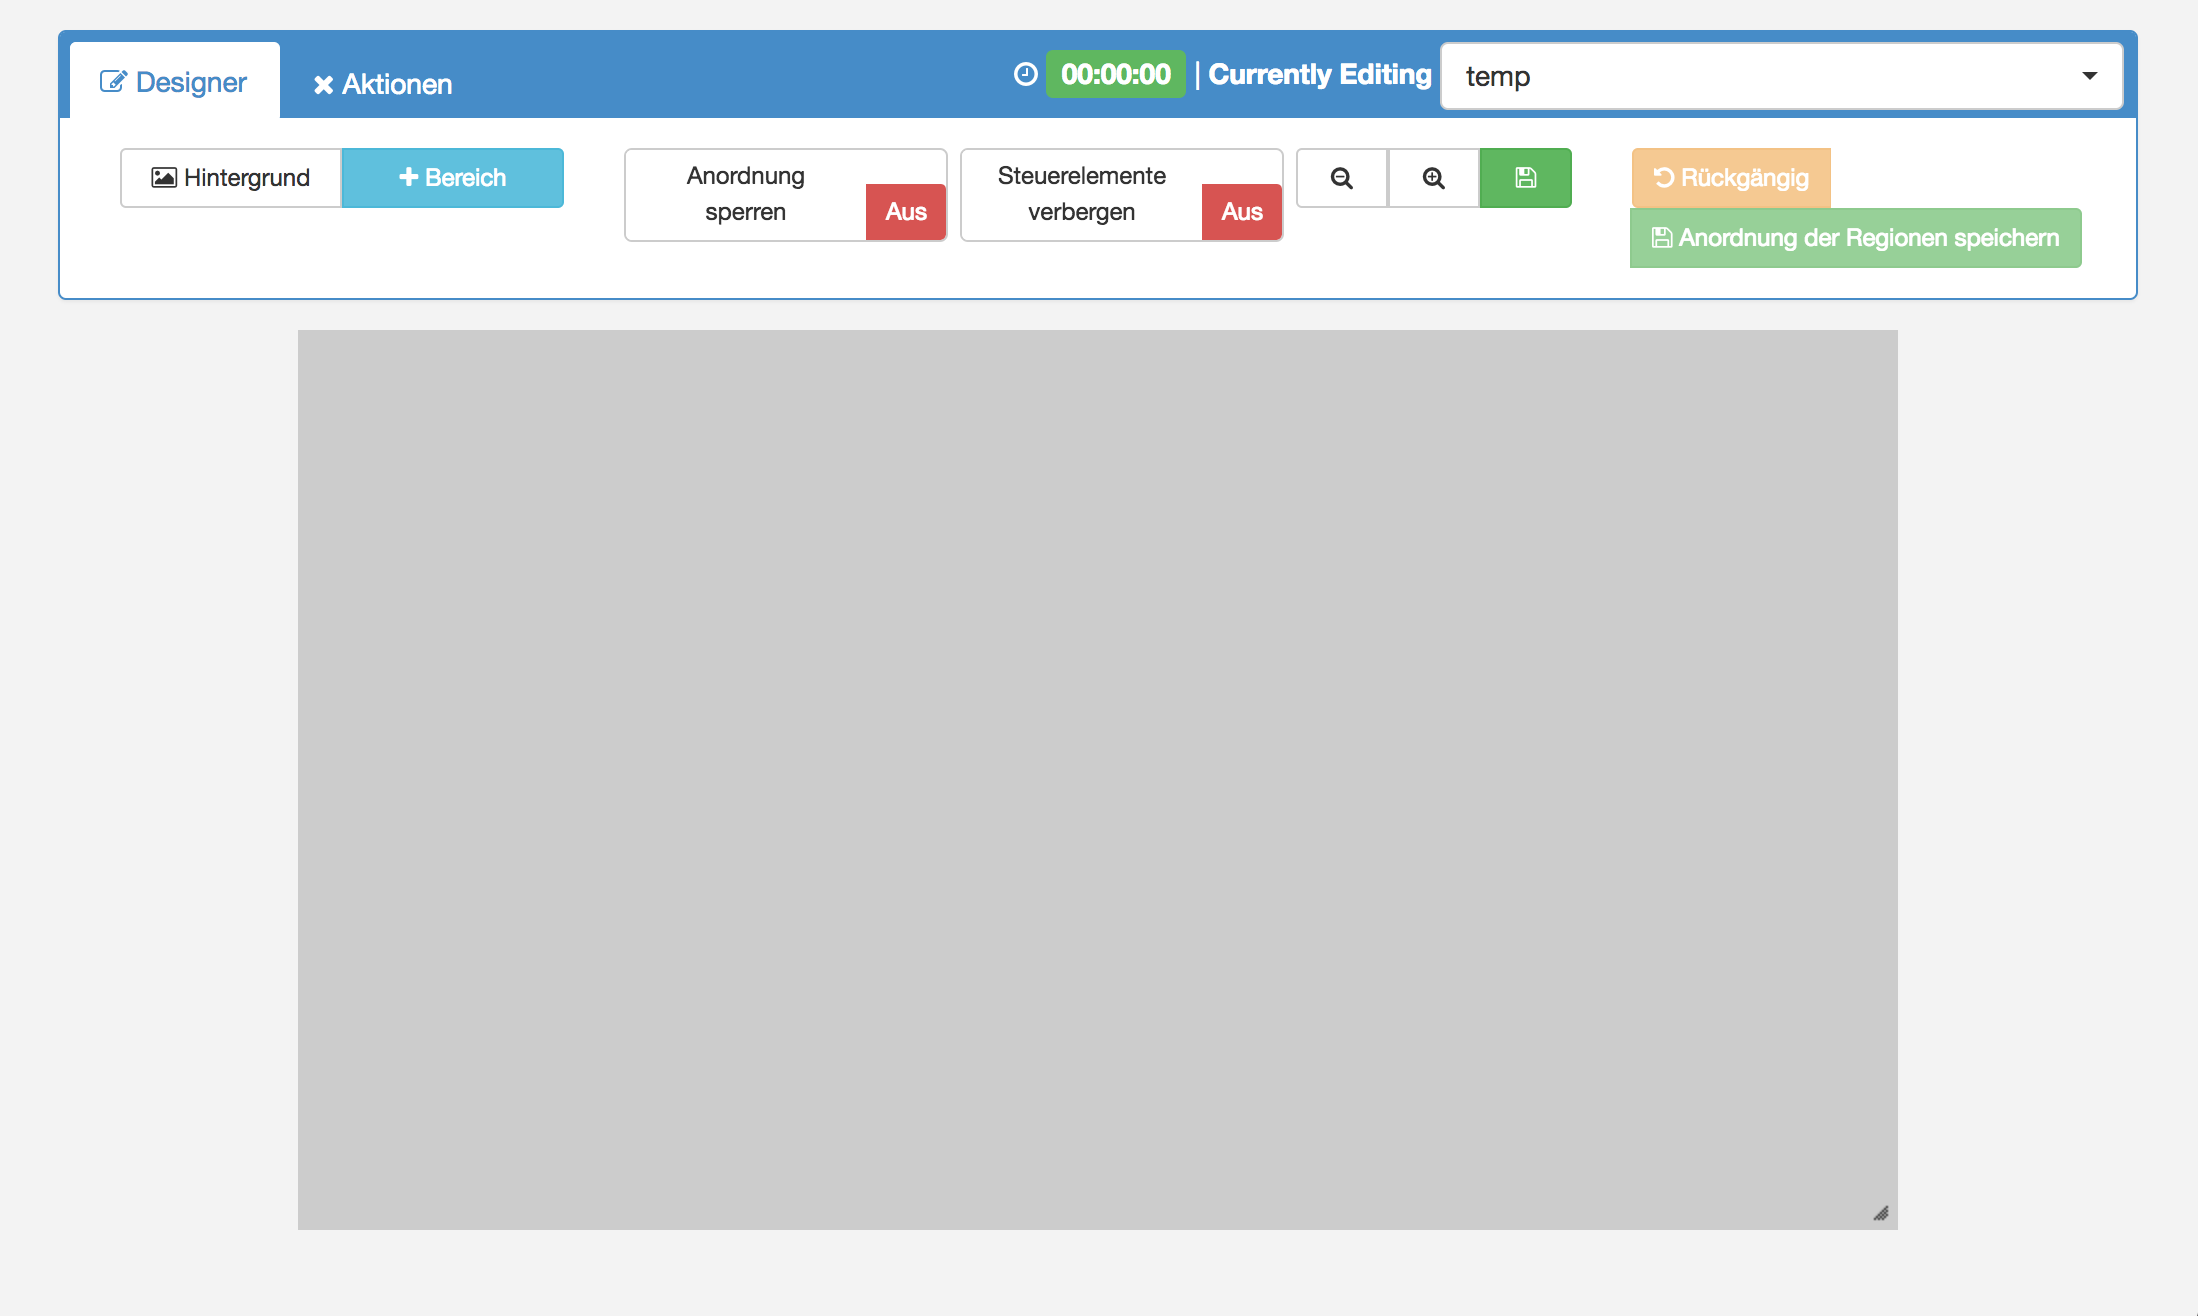
\includegraphics[width=1\textwidth]{images/xibo-basics-designer}
	\label{img:designeLayout}
	\caption{XIBO-Layout designen}
\end{calendar}	

Dem Layout kann nun eine Region oder auch mehrere  hinzugefügt werden. Eine Region kann mehrere Widgets enthalten. Mit einem Doppelklick auf die Region kann ein Widget hinzugefügt werden. Es gibt viele verschiedene Arten von Widgets:

\begin{widgettypes}
	\item {\em Bibliothek:} Mit diesem Widget können Elemente aus der Medienbibliothek in der Region angezeigt werden. Dabei werden PowerPoint Formate, Video, Bilder und andere Medien Datentypen unterstützt.
	
	\item {\em Uhr:} 
	Dieser Widgettyp bindet eine Uhr in die Region ein. Es kann entweder eine Uhr im Analogen Stil oder Digitalen Stil ausgewählt werden.
	
	\item {\em DataSet:} 
	Das DataSet Widget ist sehr wichtig und zeigt grob gesagt nacheinander Daten aus einem Array mit Key, Value Paaren an.
	
	\item {\em Wheather:} 
	Das Wheather Widget, in Deutsch Wetter, zeigt das aktuelle Wetter an. Es kann eingestellt werden ob es anhand von den GPS-Daten des Bildschirmes die Wetterdaten anzeigen soll oder ein vorher definierter Ort für die Daten verwendet werden soll.
	
	\item {\em Flash:} 
	Mit dem Flash Widget können Flash Inhalte abgespielt werden.
	
	\item {\em HLS:} 
	Mit dem HLS Widget können HLS Video Streams angezeigt werden.
	
	\item {\em Image:} 
	Mit dem Image Widget können Bilder entweder aus der XIBO Bibliothek angezeigt oder neue hochgeladen werden.
	
	\item {\em Local Video:} 
	Mit dem Local Video Widget können Videos oder Streams angezeigt werden.
	
	\item {\em PDF:} 
	Mit dem PDF Widget können PDFs entweder aus der XIBO Bibliothek angezeigt oder neue hochgeladen werden.
	
	\item {\em PowerPoint:} 
	Mit dem PowerPoint Widget können PowerPoint Präsentationen entweder aus der XIBO Bibliothek angezeigt oder neue hochgeladen werden.

	\item {\em Text:} 
	Mit dem Text Widget können Texte angezeigt werden.
	
	\item {\em Ticker:} 
	Mit dem Ticker Widget können Texte animiert angezeigt werden. Dabei können diese Texte aus einem DataSet oder einem RSS Feed stammen.
	
	\item {\em Webpage:} 
	Mit dem Webpage Widget können Webseiten angezeigt werden.
\end{widgettypes}

Nachdem eines der Widgets erstellt wurde kann das Ergebnis des Layouts mit einer Layout Vorschau kurz überprüft werden.

\chapter{XIBO-Server}
\section{Beschreibung}
Als zentrale Steuereinheit wird ein XIBO-Server verwendet. Der XIBO-Server bietet die benötigten Funktionalitäten wie zum Beispiel:
\begin{itemize}
	\item {\em Medieninhalte abspielen} 
	\item {\em Zeitsteuerung der anzuzeigenden Informationen}  
	\item {\em Verteilung der Anzeigedaten an die verbundenen Clients} 
\end{itemize}
Es gibt zwei Möglichkeiten den Funktionsumfang des XIBO-Servers zu nutzen. Zum einen über das Server interne Web-Interface, die andere Möglichkeit ist es den Server über die eingebaute REST-Schnittstelle anzusprechen.
\cite{xibo-server}
\section{API}
Die API des XIBO-Servers ist mittels Swagger dokumentiert. Diese Dokumentation deckt die Grundfunktionalitäten und die Form der Anfragen ab. Die Schnittstelle des Servers dient als wesentliches Verbindungsstück zwischen der eigens entwickelten Steuerungssoftware und dem XIBO-Server. Wie der XIBO-Server die verschiedenen Anfragen verarbeitet und entgegen nimmt wurde, bevor die Implementierung des Java-EE-Servers begonnen wurde, mittels Postman getestet. Diese Vorgehensweise war Nötig um festzustellen ob das XIBO-System über REST-API ausreichend konfigurierbar und im operativen Betrieb steuerbar ist. Die Anfragen an den Server wurden im Java Code durch die ''libary'' OkHttp3 übernommen.

\cite{swagger}
\cite{postman}
\cite{Okhttp3}
\section{Authentifizierung}

Die Authentifizierung einer Client-Applikation per REST-Anfrage am XIBO-Server erfolgt über OAuth2 , also mittels Access Token.

Zunächst ist am XIBO-Server ein ''Application''-Objekt im Webinterface zu erstellen. Beim erstellen des ''Application''-Objekts können die Berechtigungen für den Client festgelegt werden. Nachdem das Objekt erstellt wurde stellt dieses ein ''Client Secret'' zur Verfügung. Dieses ist für jeden Client eindeutig. 

Damit ein externer Client auf den XIBO-Server per REST-Request zugreifen beziehungsweise Anweisungen an diesen geben kann, wird ein POST-Request mit folgenden Parametern abgesetzt.

Die Parameter: 
\begin{itemize}
	\item {\em Client\_ID:} XIBO-Server Anwendungen neue Anwendung
	\item {\em Client\_Secret:}  XIBO-Server Anwendungen neue Anwendung
	\item{\em grant\_type:} Muss in der Form ''&grant\_type=client\_credentials''
\end{itemize}

Die über den POST-Request erhaltene Antwort liefert einen Access Token welcher 60 Minuten gültig ist und nach Ablauf erneuert werden muss um weiter über die API zu kommunizieren.
Dieser Token muss bei jedem Request an den XIBO-Server im Header des Requests übergeben werden damit der XIBO-Server feststellen kann ob es sich um einen registrierten Client handelt.

HomeDS\HomeDsBackend\src\main\java\at\htl\utils\AuthentificationHandler.java

Um den die Authentifizierung zu automatisieren wurde eine Java Klasse entwickelt. Funktionsweise dieser wird nachfolgend geschildert: 

Um eine Verbindung zum XIBO-Server herstellen zu können wird eina URL und eine HttpURLConnection deklariert. Im Anschluss wird die URL mit der richtigen Adresse belegt. Die httpURLConnection wird über den Befehl ''httpURLConnection.openConnection()'' dazu angewiesen eine Verbindung aufzubauen. Durch die Anweisung ''httpURLConnection.setDoOutput(true)'' wird der Connection mitgeteilt das als Antwort Daten erhalten werden. Die Art der Anfrage wird als POST-Request festgelegt. Um die für die Authentifizierung am XIBO-Server geforderten Parameter ''client\_id'', ''client\_secret'' und ''grant\_type'' übergeben zu können wird ein ''DataOutputStream'' deklariert und mit dem Benötigten werten versehen. Anschließend werden über den Befehl  ''DataoutputStrem.flush'' wird dem ''DataOutputStream'' mitgeteilt, dass er die Daten über die Verbindung senden soll.Um auftretende Fehler besser finden zu können werden der Übergeben Request-Body, die URL über die der Request durchgeführt wurde und der erhaltene Response-Code im Log-Fenster ausgegeben. Die Daten die anschließend vom XIBO-Server als Antwort erhalten werden, werden durch einen ''BufferedReader'', dieser bekommt bei der Instanziierung den ''InputStream'' der ''httpURLConnection'' übergeben, entgegengenommen. Solange vom Server Daten erhalten werden wird über einen ''StringBuilder'' ein String um jene erhaltenen Daten erweitert. Im Anschluss wird die ''BufferedReader'' Verbindung geschlossen und der erhaltene ''Access\_Token'' wird im Log-Fenster angezeigt. Als nächstes wird der erhaltene Token per ''return'' Statement als Ergebniss der Methode übergeben. Abschließend wird im ''finally'' Block überprüft ob die ''HttpURLConnection'' noch geöffnet beziehungsweise vorhanden ist, sollte dies der Fall sein so wird die Verbindung geschlossen.







\chapter{Verwendente Technologien}
\section{Git und GitHub}
Um dynamisch als Team arbeiten zu können, verwenden wir Software zur Versionsverwaltung. Hierbei handelt es sich um Git. 
Github ist die verwendete Online-Plattform, auf der Benutzer ihre Projekte gratis als Repository speichern. Dies ermöglicht einfaches arbeiten im Team und verhindert in den meisten Fällen Zusammenführungskonflikte. Mittels Git lässt sich auch leicht zurückverfolgen welches, Teammitglied welche Änderungen gemacht hat und im Notfall ist es auch möglich diese Änderungen wieder rückgängig zu machen.

Verwendet wird GitHub für die gesamte Diplomarbeit, sowohl für die Versionierung der Dokumente, als auch  die einzelnen Applicationen. Um sicherzustellen, das keine Konflikte durch paralleles arbeiten entstehen, wird in Branches gearbeitet. Diese Branches wurden erstellt, wenn ein neues Arbeitspaket begonnen wurde, zum Beispiel die Android-App.

Bild Github und verweis Git/GitHub

\section{Android}

Android ist ein Betriebssystem für mobile Endgeräte, spezialisiert für Touch-Anwendungen. Ziel ist es das Endgerät möglichst intuitiv und flexibel bedienen zu können. Mit Android ist es möglich open-source Applicationen zu erstellen die ein großes Publikum erreichen. Google stellt auch einen Markt zur Verfügung in dem die Applicationen gratis oder auch gegen Entgelt erworben werden können.
Diese Aspekte: open-source, gratis und großes Publikum, waren ausschlaggebend dafür, dass die Applicationen in Android implementiert wurden. Als Programmiersprache wurde JAVA verwendet.




\section{Java Enterprise Edition}\label{sec:javaee}
Java Platform, Enterprise Edition oder abgekürzt auch Java EE ist die technische nähere Beschreibung einer Softwarearchitektur, die programmierte Java Anwendungen ausführt.
(weiter ausführen)

QUELLE: https://de.Wikipedia.org/wiki/Java_Platform,_Enterprise_Edition
\chapter{HomeDS - Server}
\section{Einleitung}\label{sec:einleitung}
Im Rahmen der Diplomarbeit wird neben dem XIBO-Server ein weiterer Server eingesetzt. Es handelt sich um einen Java Enterprise Edition Server. Aufgrund der hohen komplexität des Signage-Servers aber jedoch dünn dokumentierten API-Schnittstellen und begrenzten technischen Möglichkeiten, muss ein eigens programmierter Server eingesetzt werden. Dieser wird die Kommunikation vom Signage Server zur Android App erleichtern. Der JavaEE Server verwendet die Funktionen des Signage Servers und baut diese meist aus sodass neue Funktionen entstehen können.

GRAFIK KOMMUNIKATION
 
\section{Anforderungen an den HomeDS Server}\label{sec:homeds}
Der JavaEE Server soll die verschiedenen komplizierten Abläufe des XIBO-Servers vereinfachen. Die  Zugriffe mittels REST die eigentlich direkt auf den XIBO laufen sollen, werden über den JavaEE Server verwaltet. Das heißt der Java Enterprise Server empfängt REST Zugriffe verarbeitet diese entsprechend und tätigt dann REST Abfragen auf den XIBO Server. Dies hat insofern Vorteile, da die komplizierten und meist mit viel Aufwand verknüpften Authentifizierungen wegfallen. Somit können ohne Probleme neue Funktionen hinzugefügt und neue Anforderungen flexibel erfüllt werden. Unser System erweitert  den Signage Server.
 
\section{Komponenten des HomeDS Server}\label{sec:homedscomponents}
Der JavaEE Server verfügt über eine eigene MySQL Datenbank. Diese wird benötigt, um Nachrichten Pakete und Kampagnen' aus dem Signage-Server zwischenzuspeichern. Diese Nachrichten Pakete auch DataSets genannt enthalten einen Titel und eine Nachricht die dann angezeigt werden. Des weiteren ist auf dem Server auch eine JSF also Java Server Faces Komponente dabei. Diese gibt den Nutzern die Möglichkeit über die HomeDs Webseite alle Funktionen des Server zu nutzen. Der ganze Server wird auf einem Wildfy Application Server mittels Continous Integration deployed. 
 
\section{Funktionen des JavaEE}
\subsection{DataSet mit Ablaufdatum}\label{sec:datasetexpiredate}
Eine der Funktionen des Servers ist das Hinzufügen, Ändern und Löschen von DataSets. Da der Digital Signage Server über keine Zeitsteuerung der Nachrichten Pakete verfügt musste diese Funktion auf den JavaEE Server ausgelagert werden.

Der Benutzer kann Start- und Enddatum für jeden einzelnen DataSet eingeben. Erst wenn das Datum genau in diesem Zeitintervall inklusive den Grenzen liegt, wird das DataSet an den Xibo mittels API-Schnittstelle weitergegeben. Es wurde auch so programmiert das bei keinem Startdatum das Nachrichten Paket sofort angezeigt wird oder wenn kein Enddatum festgelegt wird das es bis zum Manuellen deaktivieren angezeigt wird.

\begin{lstlisting}[language=Java, caption={public void doCheckEvery24Hours()}]
if (dataset.isActive() == false && (dataset.getFromDate().minusDays(1)
        .isBefore(LocalDate.now()))) {
    try {
        //if succesfull added then set active true and add id
        if ((id=dataSetApi.addDataSetField(dataset)) > 0) {
            dataset.setDataRowId(id);
            dataset.setActive(true);
            dataSetFieldFacade.save(dataset);
        }
    } catch (NoConnectionException e) {
        // Catch Exception
    }
}
\end{lstlisting}

Die Überprüfung ob die DataSets aus der Server-Datenbank im Zeitintervall liegen, wird mithilfe der Java Annotation @Schedule jeden Tag um 01:00 Uhr durchgeführt. Falls dieses DataSet im Intervall liegt, wird dieses an den XIBO Signage Server gesendet. Diese Überprüfung beinhaltet auch das FromDate. Dies löscht bei überschreiten des Bis-Datums das DataSet aus dem Digital Signage heraus. Solange das DataSet sich im XIBO befindet wird es angezeigt nach dem entfernen aus dem XIBO wird es dann auch nicht mehr angezeigt.

Falls keine Nachrichten Pakete aktiv oder im System sind werden aus dem RSS-Feed der HTL Leonding die Neuigkeiten anstatt der Nachrichten Pakete angezeigt.

\subsection{Medien abspielen}\label{sec:playmedia}
Eine weitere Funktion des Servers ist das abspielen von Medien auf einen bestimmten Bildschirm. Dabei muss im XIBO ein definiertes Layout erstellt werden mit einer absoluten Id. In diesem Layout wird eine Region über die volle Auflösung erstellt die ein Bibliothek Widget enthält. Diesem Widget wird dann per REST das vom Nutzer ausgewählt Medium eingefügt. Sobald diese Operationen erfolgreich ausgeführt wurden wird per REST das definierte Layout auf den vom Nutzer ausgewähltem Bildschirm eingeplant.

\subsection{Jave Enterprise Edition mit Android über REST}\label{sec:javaeeandroidrest}
Ein weiterer Teil des Server auf Java Enterprise Edition Basis ist die Kommunikation mittels REST. Alle Funktionen des Servers werden per REST zur Verfügung gestellt.

\section{Swagger}\label{sec:javaeeandroidrestswagger}
Swagger wird verwendet um Funktionalität und Möglichkeit einer API übersichtlich zu gestalten. Dabei gibt es zwei verschiedene Arten eine REST-Dokumentation zu erstellen.
Dabei dokumentiert Swagger welche Response Code's man erwarten kann wie bei einem POST oder PUT der Body aussehen muss oder welche Pathparams mitgegeben werden müssen und welche nur optional sind.  

Die erste Möglichkeit wäre, mit dem Swagger Editor die Dokumentation in der JSON-Ausdruckssprache mit der Hand zu schreiben und immer wieder zu aktualisieren. Natürlich ist dies bei vielen verschiedenen GETs, POSTs, PUTs und DELETEs sehr aufwendig und mühsam.

Bei der zweiten Methode, die auch bei der Diplomarbeit zum Einsatz kommt, werden die API's automatisch von der im Projekt eingebundenen Swagger Engine erkannt. Daraus wird dann auch wieder eine JSON-File generiert, die dann mithilfe von Swagger-UI gut im Browser über eine Webseiten URL erreichbar ist.


Verweis: https://swagger.io/

\section{Java Server Faces mit JavaEE}\label{sec:javaeejsf}
Um den Benutzern die Möglichkeit zu geben die Funktionen unseres Servers zu nutzen wurde im Rahmen der Diplomarbeit auch eine Webapplikation erstellt. Und da JSF also Java Server Faces mit einem Java EE Server harmoniert haben wir uns entschieden solch eine Webapplikation zu erstellen. Dies hat viele Vorteile wie z. Bsp. die Platformunabhängigkeit und auch die schnelle Entwicklung im Vergleich zu anderen Clients. 

Mit JSF wird nämlich über eine Managed Bean direkt im XHTML auf die Funktionen des Servers zugegriffen somit sind keine REST Zugriffe nötig.

\begin{figure}[h]
\centering
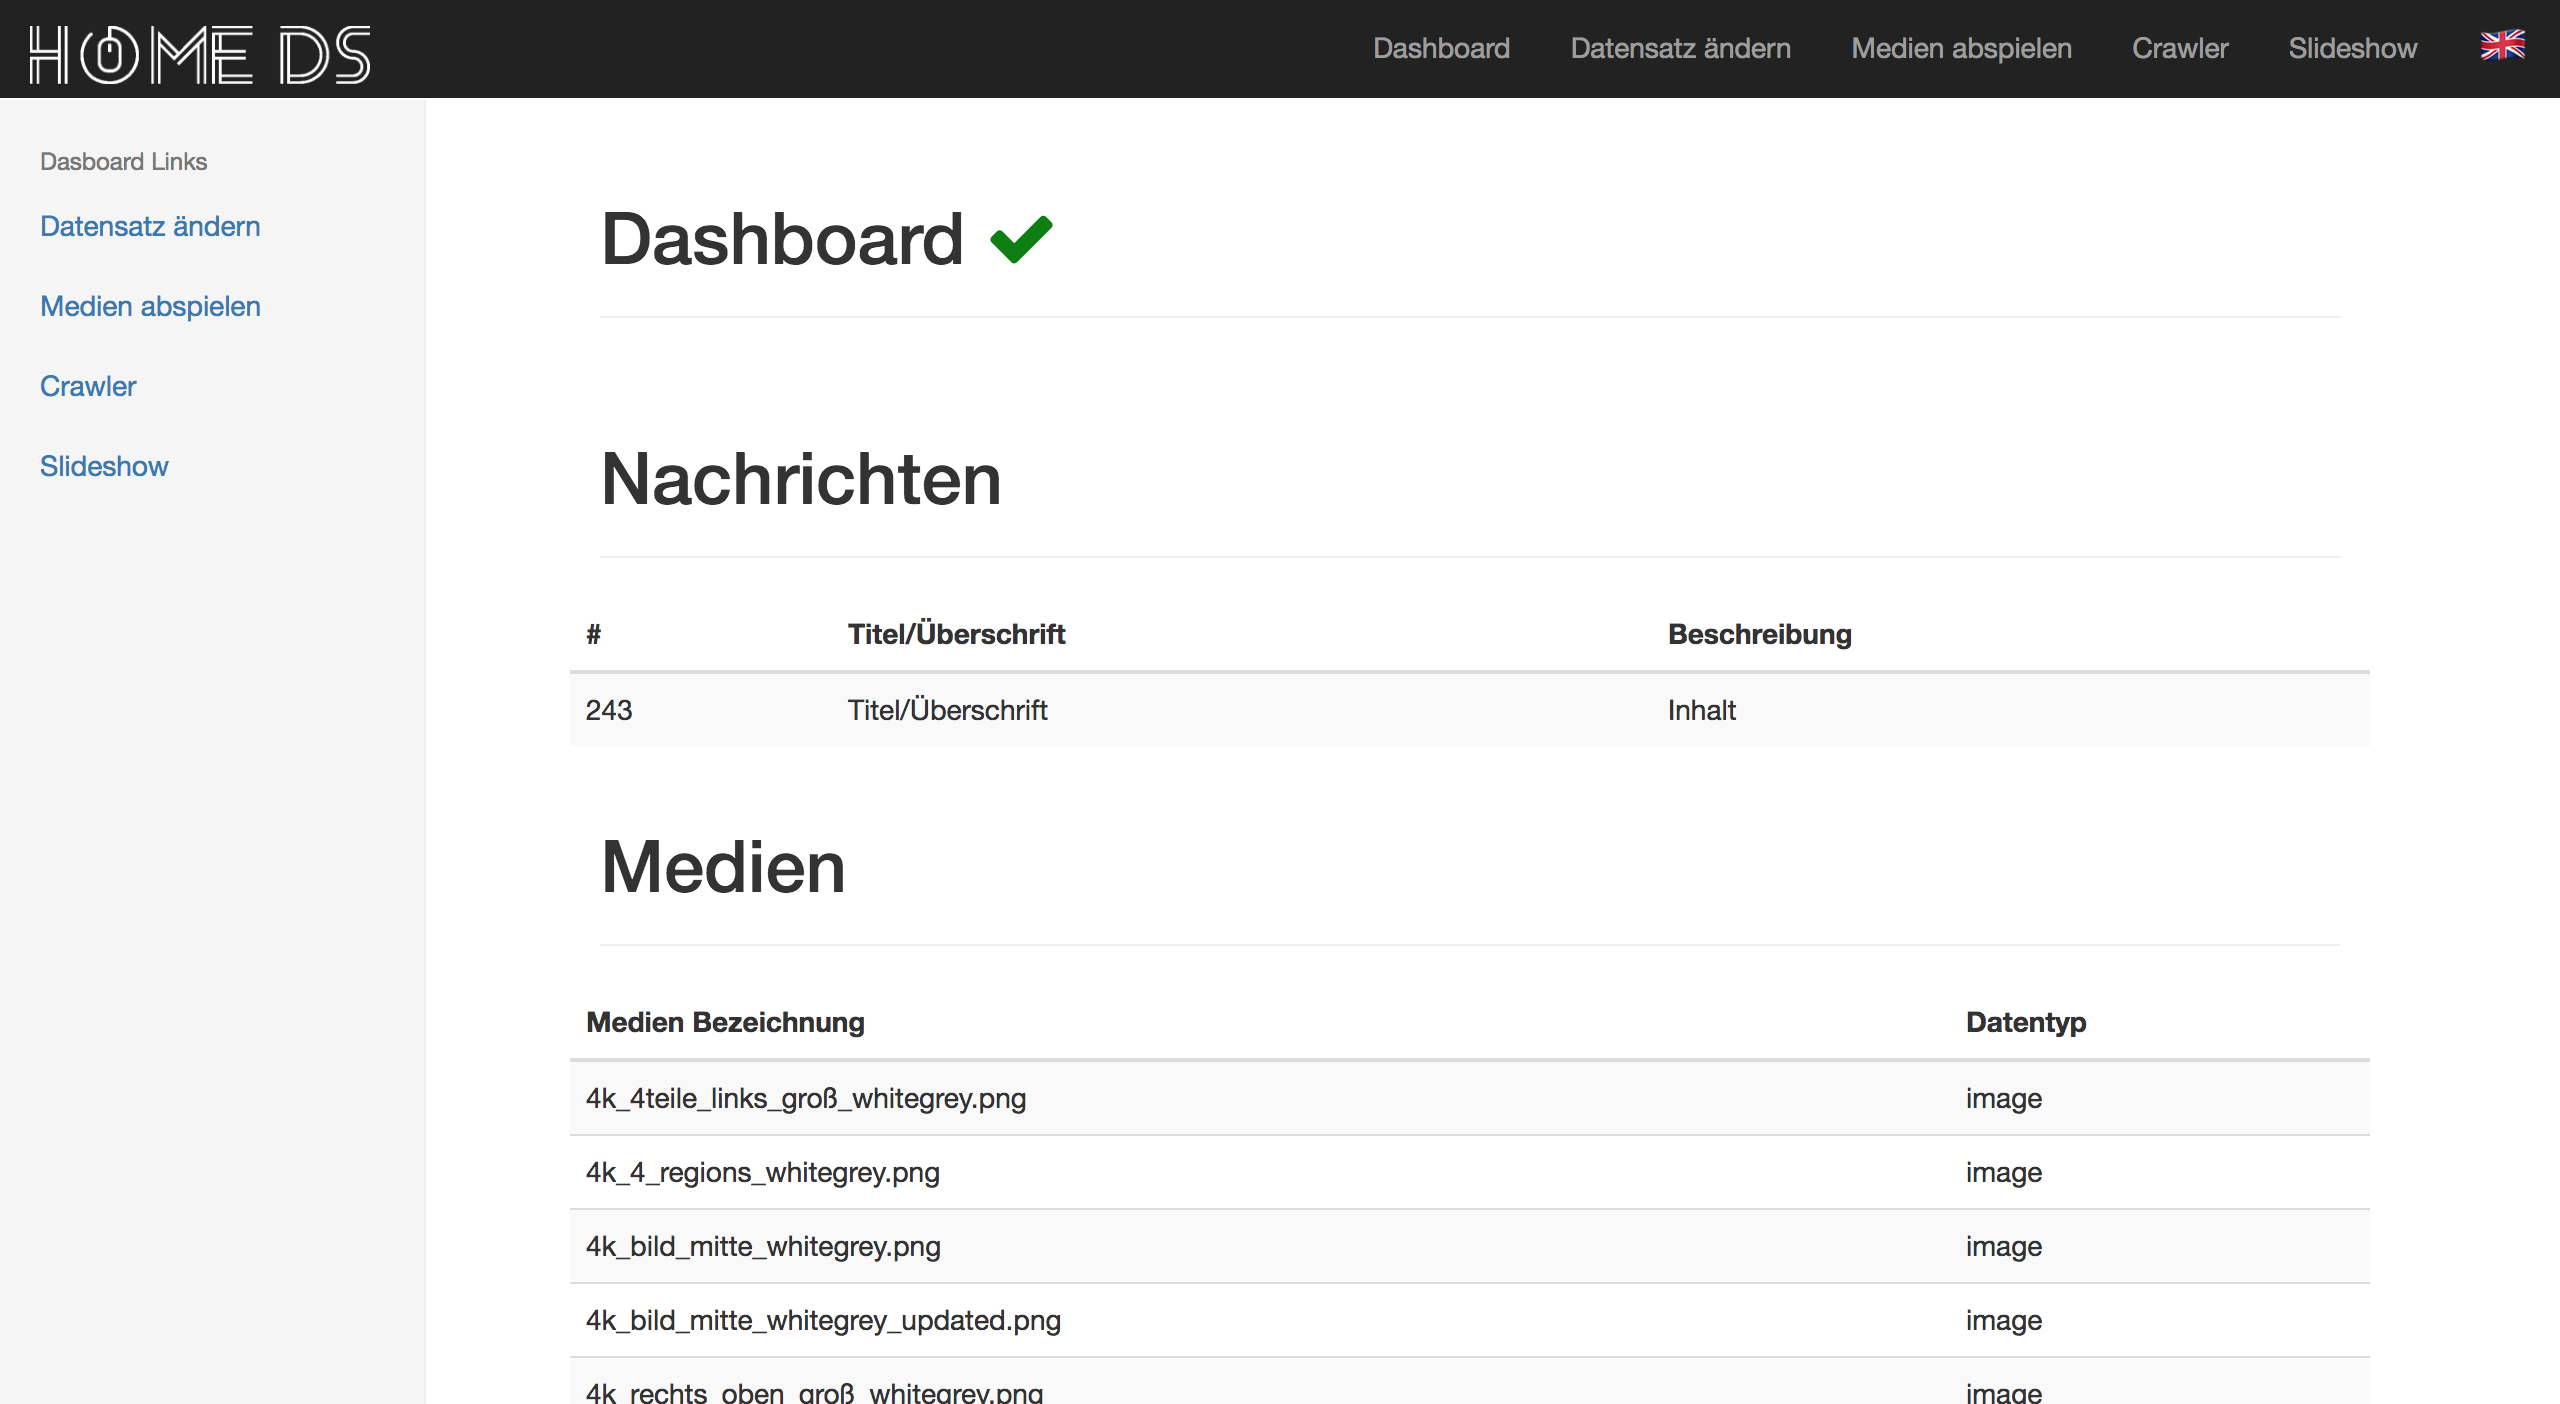
\includegraphics[width=1\textwidth]{images/08_HomeDsWeb/DashboardHomeDsWeb.png}
\caption{Startseite - HomeDsWeb}
\label{img:Startseite}
\end{figure}

Unsere Weboberfläche ist Responsive gestaltet und mithilfe von Java Server Faces mit BootsFaces realisiert worden. Das Bootsfaces Framework stellt fertige Komponenten zur Verfügung wie Buttons, Listen, Forms etc. Dabei wurde Bootstrap als Vorbild hergenommen.

Uns war es wichtig die Oberfläche so zu gestalten das diese übersichtlich und leicht zu bedienen ist. Das Designen wurde mit enger Zusammenarbeit mit dem zukünftigen Benutzern der Software ausgearbeitet. Als Vorbild fungierte mehr oder weniger ein Cockpit eines Flugzeuges wo vielen Funktionen direkt bei der Hand liegen müssen und trotzdem alles seine Ordnung hat. In der Abbildung \ref{img:Startseite} ist das Dashboard abgebildet. 
Hier erkennt man nun das es sich um die Kommandozentrale der Applikation handelt von dieser Seite aus kann man über eine Top-Navigationsleiste oder Left Sidebar Navigation zu allen Funktionen des Server gelangen. 

Um den Nutzer immer ein Feedback über den aktuellen Status der Verbindung vom XIBO zu JavaEE Server zu geben wird bei Erfolgreicher Verbindung ein grünes Häkchen visualisiert versehen mit eine Tooltip. Oder bei keiner Verbindung zum Server ein rotes x dargestellt wie in Abbildung  /ref(img:NoConnection}.

\begin{figure}[h]
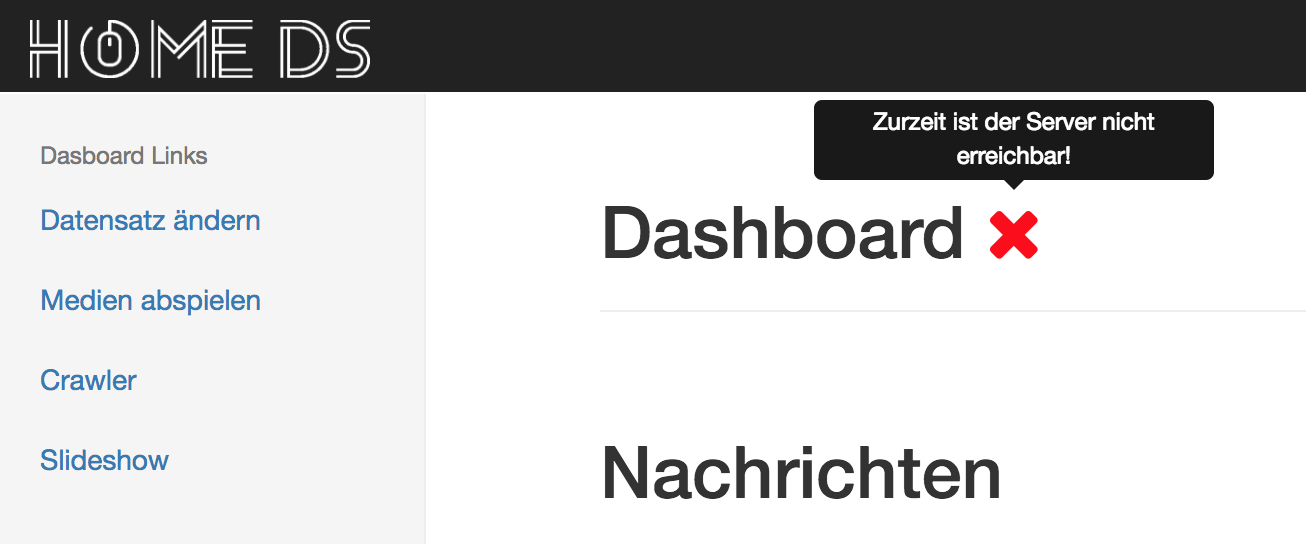
\includegraphics[width=1\textwidth]{images/08_HomeDsWeb/DashboardNoConnection.png}
\caption{Keine Verbindung zum XIBO - HomeDsWeb}
\label{img:NoConnection}
\end{figure}

\section{Nachrichten Pakete ändern - HomeDS Web}\label{sec:homedswebdataset}
Die Datensatz ändern Funktion auch genannt Nachrichten Pakete ändern, DataSet bearbeiten oder Nachrichten Pakete bearbeiten kann über das Dashboard erreicht werden.
Die Aufgabe der DataSet Webapplikation ist ein DataSet zu ändern, hinzufügen oder zu löschen. Die Applikation besteht grob gesagt aus 2 Teilen. Diese 2 Teile können bei Bedarf auf- und zugeklappt werden.

Teil 1 kümmert sich um das Anzeigen aller DataSets in einer Responisve Komponente die "DataTable" gennant wird in der Bibliothek vom Bootsfaces Framework. Im DataTable ist es möglich die Anzahl der angezeigten Elemente pro Seite zu begrenzen oder erweitern,  die einzelnen Spalten sortieren dabei kann man zwischen ab- oder aufsteigend wählen und durch die verschiedenen Spalten einer Zeile eine Suche durchzuführen. 

Es ist auch durch die editierbaren Textfelder und DatePicker möglich die DataSets zu ändern. Durch klicken auf den Speichern Button wird die Änderung des einzelnen DataSets bestätigt. Durch klicken auf den roten Löschen Button wird das Nachrichtenpaket gelöscht falls es aktiv war wird es auch aus dem XIBO System entfernt. Die Logik ist im /pageref{sec:datasetexpiredate} nochmals genauer erklärt. 

Der zweite Teil der Datensatz ändern Seite ist das Hinzufügen von Nachrichtenpaketen. Dabei ist der Titel und der Inhalt der Nachricht natürlich erforderlich. Bei nicht eingeben von Start Datum des Nachrichtenpakets wird davon ausgegangen das es sofort in den XIBO gespeichert werden soll und somit auf aktiv gesetzt wird. Andersrum wenn kein Ablaufdatum eingegeben wird, wird das DataSet solange angezeigt bis entweder ein Ablaufdatum im Nachhinein hinzugefügt wird oder es manuell einfach wieder gelöscht wird.

Nach jeder Aktion bekommt der Nutzer ein Feedback ob die jeweilige Operation erfolgreich oder fehlgeschlagen

Verweis auf JSF Section,


\section{Medien abspielen}\label{sec:playmedia}
Eine weitere wichtige Funktion ist das Abspielen der Medien die im XIBO hinterlegt sind. Es soll dem Nutzer eine einfache und übersichtliche Oberfläche zur Verfügung gestellt werden die Medien abspielen soll. Der Nutzer kann jedoch vorher den Bildschirm auswählen auf den diese Medien abgespielt werden sollen. Um jedoch zu verhindern das der Nutzer zwischen hunderten von Medien sein Video suchen muss gibt es eine Schlagwort Wolke.

Die Medien im XIBO sind mit einem Schlagwort versehen. Diese Schlagwörter können sein die jeweilige Abteilung also Informatik, Medientechnik oder Elektronik. Oder aber auch ob es sich um ein Projekt oder sonstiges. 

Mithilfe dieser Tags wollen wir dem Nutzer die Suche nach dem richtigen Video erleichtern. Der Nutzer bekommt die Möglichkeit einer dieser Tags auf der HomeDs Weboberfläche auszuwählen daraufhin werden nur die Videos mit dem entsprechendem Tag angezeigt.


\section{HomeDS Server Projekt-Struktur}\label{sec:javaeestruktur}


\section{HomeDS Server Structure Crawler}\label{sec:javaeestructurecrawler}
Für das verstehen des Aufbaus eines Layouts war es die Aufgabe einen sogennanten StructureCrawler zu erstellen. Dieser soll den JSON Aufbau eines Layouts ausgeben. Durch diese Funktion ist es für uns möglich gewesen das ganze Signage System zu verstehen und zu verwenden. Der Crawler ist eigentlich nur ein REST-Zugriff der sich alle Layouts vom XIBO Server holt und dabei alle anderen Child-Elemente des Layouts mitschickt. Dies ist praktisch den es unterstützt uns bei dem Arbeiten mit vielen verschiedenen Ids die richtig sein müssen.

WEBOBERFLÄCHE VOM CRAWLER

\section{HomeDS Server Slideshow}\label{sec:homedsslideshow}
Eine weitere Funktion des HomeDs Servers ist das abspielen von Medien ohne diese in den XIBO hochladen zu müssen. Dies ist insofern wichtig da man bei großen Mengen von Daten nicht das XIBO zu müllen sollte. Dies wurde mittels JSF, Bootsfaces und JavaScript realisiert. Die Bilder werden von einem lokalen Ordner der Reihe nach abgespielt. Der Wechselintervall beträgt 3 Sekunden.

JavaScript	code erklären

\chapter{Android Application}
\section{Einleitung}

\begin{figure}[H]
\centering
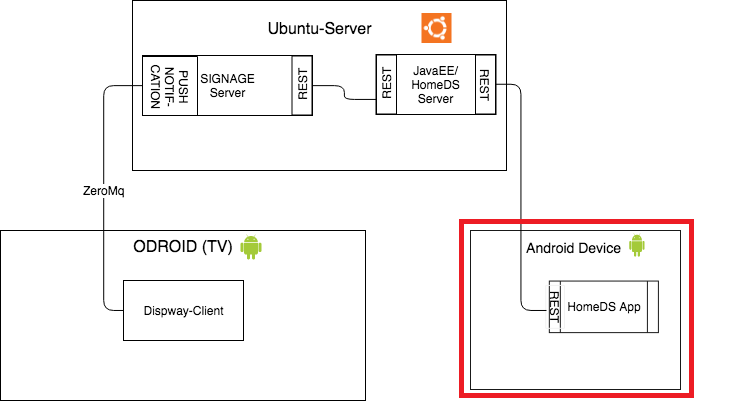
\includegraphics[width=1.0\textwidth]{images/06_AndroidApp/06_SystemArch}
\caption{Die Android Applikation dient zur mobilen Benutzung}

\end{figure}
\\
Um eine höchst mögliche Reichweite an Endgeräten zu erzielen, wurde eine Android Applikation entwickelt, mit der die wichtigsten Funktionen abgedeckt werden. Zum Beispiel das Wechseln der DataSets des XIBO-Servers. Wichtig war es die Applikation möglichst einfach und leicht bedienbar zu gestalten, um auch Erstbenutzern die Bedienung zu erleichtern. 
Prototyp für die aktuelle Applikation war eine Anwendung für Android, die direkt mit dem Digital Signage Server kommuniziert. Es stellte sich heraus, dass das Steuern des Servers direkt über eine Applikation auf Android Basis viel zu umständlich ist, wurde eine Browser Applikation entwickelt, welche über das ''HomeDsBackend''(Java-EE-Server) kommuniziert, um das Funktionsspektrum zu erweitern und die Applikation möglichst kompakt zu gestalten. Beispielsweise ist es durch diese Aufteilung nicht mehr nötig eine Datenbank in der Applikation zu haben. Somit erleichtert es auch Applikationen für andere Betriebssysteme zu implementieren. 
\section{Anforderungen}
\\
\begin{figure}[H]
\centering
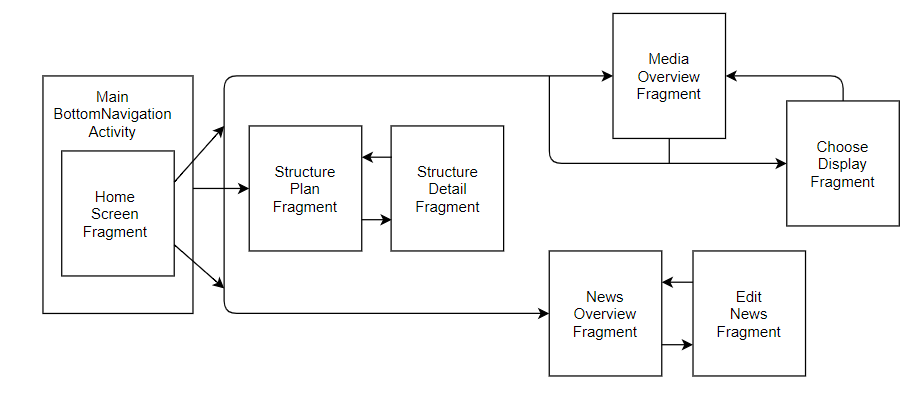
\includegraphics[width=1.0\textwidth]{images/06_AndroidApp/06_AndroidArch}
\caption{Fluss Diagramm der Android Anwendung}
\label{fig:mediaNav}
\end{figure}
\\
Die Anforderungen an die Android Applikation weichen von den Anforderungen an das ''Backend'' leicht ab, da das ''Backend'' die gesamte Zeitsteuerung- und Datenbankfunktionalität übernimmt. Es besteht die Möglichkeit, den Server über die Website des ''Backend'' zu steuern, beziehungsweise über die Applikation auf Android Basis. 
\begin{itemize}
	\item {\em Eilmeldungen:} Dem Benutzer soll es möglich sein Nachrichten in einem Ticker auf den Bildschirmen anzuzeigen.
	
	\item {\em Medien Wiedergabe:} Medien die Lokal am Digital Signage Server liegen sollen abgespielt werden können.
		
	\item {\em Authentifizierung automatisieren (Prototyp Applikation):} Die Authentifizierung am Digital Signage Server soll automatisiert werden, um nicht vom Benutzer durchgeführt werden zu müssen.  		
\end{itemize}
\section{Struktur}
\begin{itemize}
	\item {\em activity:} Alle Activities die für die Anwendung benötigt werden. Als Beispiel die MainActivity
	
	\item {\em adapter:} Hier befinden sich alle Adapter für die RecyclerViews.
	
	\item {\em apiClient:} Beinhaltet die Klasse ''RequestHelper'' mit der die Anfragen an den Digital Signage Server beziehungsweise an das HomeDsBackend vereinfacht werden.
	
	\item {\em entity:} Jene Klassen die als Models für die Anwendung benötigt werden. 
		
	\item {\em enumeration:} Enumerationen welche die Android Basierte Applikation verwendet. Zum Beispiel das ''RequestTypeEnum''.
	
	\item {\em fragment:} Alle Fragments die für das User Interface benötigt werden. Beispiel hierfür ist das Fragment ''NewsOverviewFragment'', welches alle DataSets die am Server sind anzeigt.
	
	\item {\em viewholder:} Beinhaltet alle ''ViewHolder'' die für die Verschiedenen ''RecyclerViews'' benötigt werden. 		
\end{itemize}
\section{Benutzerhandbuch}
\subsection{Startseite}
Auf der Einstiegsseite der Applikation ist ein Feld mit dem Serverstatus zu sehen sollte dieses Rot eingefärbt sein gibt es Verbindungsprobleme zum Server(die Applikation kann keine Daten vom Server erhalten oder Daten an den Server senden) andernfalls kann mit der Benutzung fortgefahren werden, des Status wird grün Angezeigt. Die Funktion der Beiden Buttons wird im weiteren velauf des Benutzerhandbuchs erklärt.
\\
\begin{figure}[H]
\centering
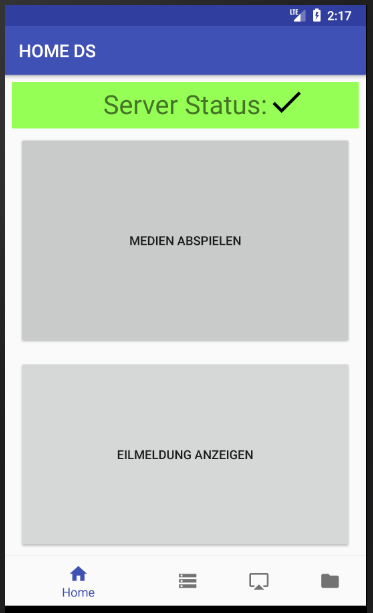
\includegraphics[width=1.0\textwidth]{images/06_AndroidApp/06_StatusOnline}
\caption{Startseite mit Status Element Online}
\label{fig:mediaNav}
\end{figure}
\\
\\
\begin{figure}[H]
\centering
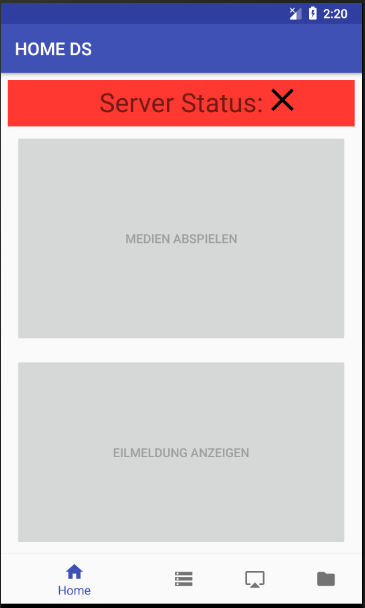
\includegraphics[width=1.0\textwidth]{images/06_AndroidApp/06_StatusOffline}
\caption{Startseite mit Startseite mit Status Element Offline}
\label{fig:mediaNav}
\end{figure}
\\
\subsection{Abspielen von Medien auf gewünschten Bildschirmen}
Das Abspielen von Medien wird im Navigationstab ''Play Media'' abgewickelt, des weiteren befindet sich auf der Startseite ein Button über den direkt zu dieser Sektion navigiert werden kann.
\\
\begin{figure}[H]
\centering
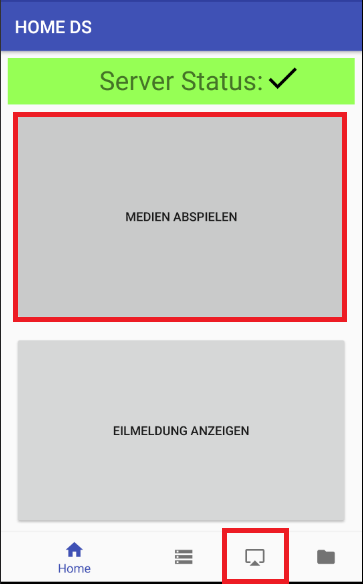
\includegraphics[width=1.0\textwidth]{images/06_AndroidApp/06_mediaNavigation}
\caption{Startseite mit markierten Navigationselementen}
\label{fig:mediaNav}
\end{figure}
\\
Wurde noch kein Display gewählt, auf dem das Medium abgespielt werden soll, erscheint zu beginn eine Auswahlmaske für die Bildschirme die verfügbar sind. Nach Auswahl einer Anzeige navigiert die Applikation automatisch zur Medienübersicht. Ist bereits ein Bildschirm ausgewählt wird direkt eine Übersicht der abspielbaren Medien angezeigt. Im rechten oberen Teil der Ansicht ist der Gewählte Bildschirm zu sehen und über einen Button wird die Bildschirmauswahl angezeigt.
\\
\begin{figure}[H]
\centering
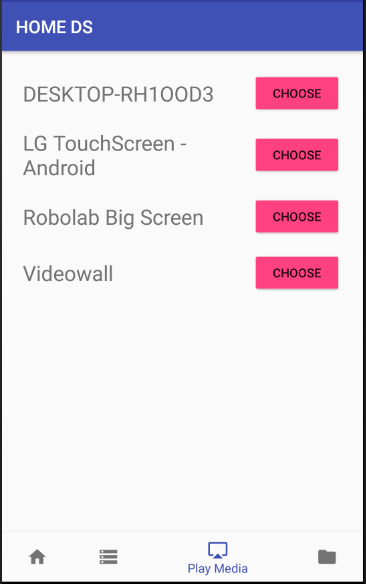
\includegraphics[width=1.0\textwidth]{images/06_AndroidApp/06_displayChoice}
\caption{Liste mit verfügbaren Displays}
\label{fig:mediaNav}
\end{figure}
\\
\begin{figure}[H]
\centering
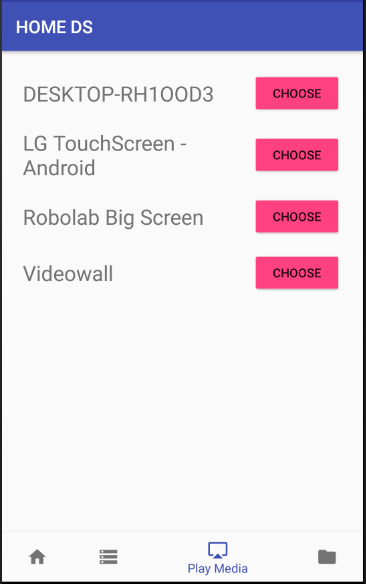
\includegraphics[width=1.0\textwidth]{images/06_AndroidApp/06_displayChoice}
\caption{Ausgewählter Bildschirm und Button für die Auswahl}
\label{fig:mediaNav}
\end{figure}
\\
Sortieren der angezeigten Medien ist über einen Spinner im linken oberen Teil der Medien Übersicht möglich durch Berührung der Anzeigefläche erscheint die Auswahl der Sortiervorschläge.
\begin{figure}[H]
\centering
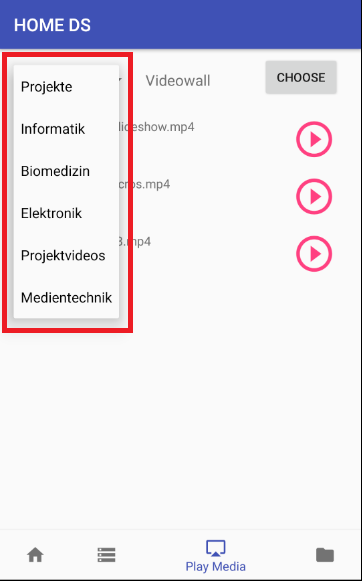
\includegraphics[width=1.0\textwidth]{images/06_AndroidApp/06_TagChoice}
\caption{Spinner mit Tags zur Sortierung}
\label{fig:mediaNav}
\end{figure}
\\
Um ein in der Liste angezeigtes Medium abzuspielen muss der Play-Button im rechten teil des Listenelements gedrückt werden. Wurde der Button betätigt wird das Medium auf der gewählten Anzeige abgespielt.
\begin{figure}[H]
\centering
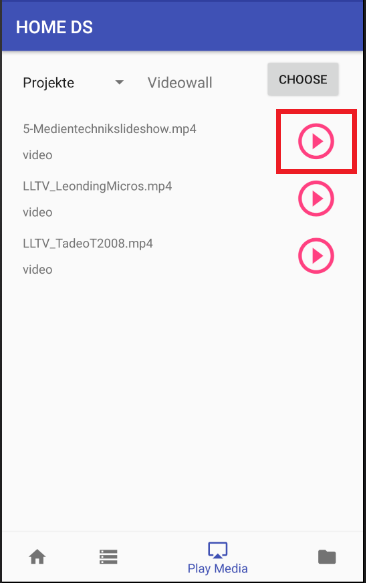
\includegraphics[width=1.0\textwidth]{images/06_AndroidApp/06_playMedia}
\caption{Play Button um Medium abzuspielen}
\label{fig:mediaNav}
\end{figure}
\\
\subsection{Meldungen Anzeigen}
Um eine Meldung anzuzeigen muss zum ''DataSet'' Tab gewechselt werden dies ist auch über eine Schaltfläche auf der Startseite von statten gehen.
\begin{figure}[H]
\centering
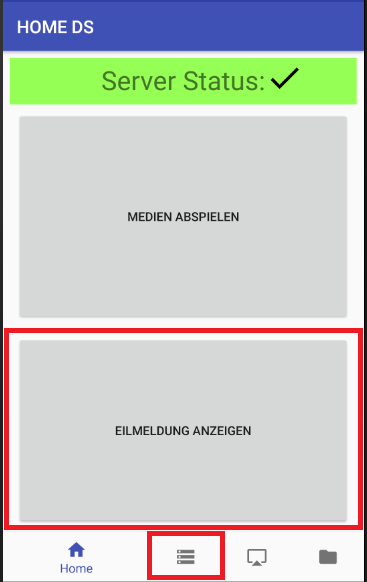
\includegraphics[width=1.0\textwidth]{images/06_AndroidApp/06_dataSetNavigation}
\caption{Startseite mit Navigationselementen}
\label{fig:mediaNav}
\end{figure}
\\
Die im der Ansicht zu sehende Liste enthält alle aktiven und  inaktiven Meldungen die auf den Anzeigen wiedergegeben werden beziehungsweise werden können. 
\\
Bild 
\\
Durch auswählen eines der Listenelemente öffnet sich einer Detailansicht über die die Informationen der Meldung verändert werden können zum Beispiel der Titel oder der Anzeigezeitraum. Wird der FloatingActionButton im unteren rechten teil der Ansicht gedrückt so öffnet sich ein Detailfenster welches noch keine Daten eingetragen hat um eine neue Meldung zu erstellen.
\begin{figure}[H]
\centering
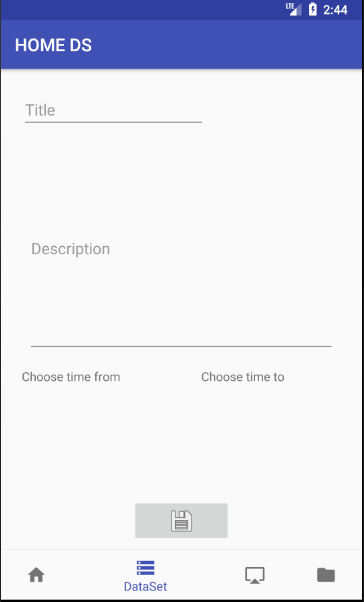
\includegraphics[width=1.0\textwidth]{images/06_AndroidApp/06_NewNewsEdit}
\caption{Anzeige bei Erstellung einer anzuzeigenden Nachricht}
\label{fig:mediaNav}
\end{figure}
\\
\begin{figure}[H]
\centering
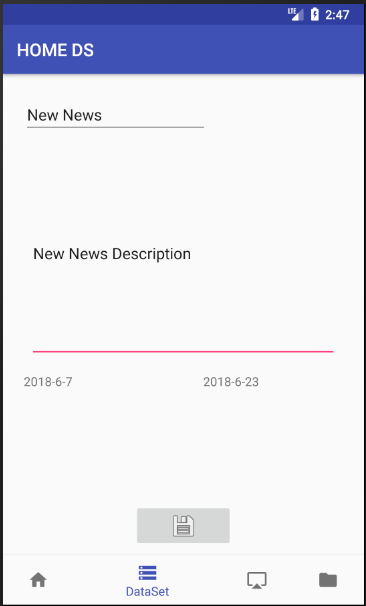
\includegraphics[width=1.0\textwidth]{images/06_AndroidApp/06_EditNews}
\caption{Anzeige bei Veränderung einer anzuzeigenden Nachricht}
\label{fig:mediaNav}
\end{figure}
Vorgenommene Änderungen oder neu erstellte Meldungen können mittels Save Button übernommen werden. Dieser befindet sich im unteren teil der Detailansicht. Nach speichern einer Meldung navigiert die Applikation wieder auf die Übersicht der Meldungen.

\begin{figure}[H]
\centering
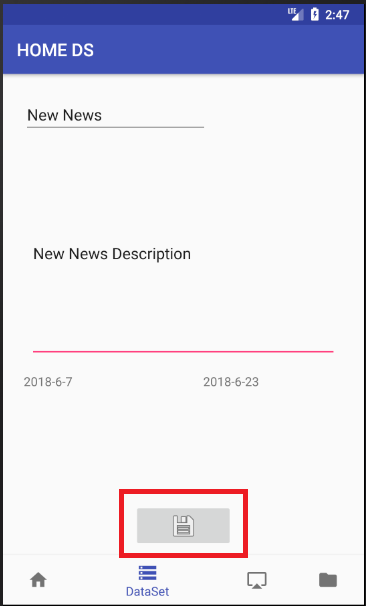
\includegraphics[width=1.0\textwidth]{images/06_AndroidApp/06_EditNewsSaveButton}
\caption{Markierter speichern Button}
\label{fig:mediaNav}
\end{figure}

\subsection{Strukturübersich}
Ist es von Nöten eine detailierte Übersicht über die am Server liegenden Layouts zu bekommen kann dies über den Navigationstab ''Structure Plan'' getan werden. 
\\
\begin{figure}[H]
\centering
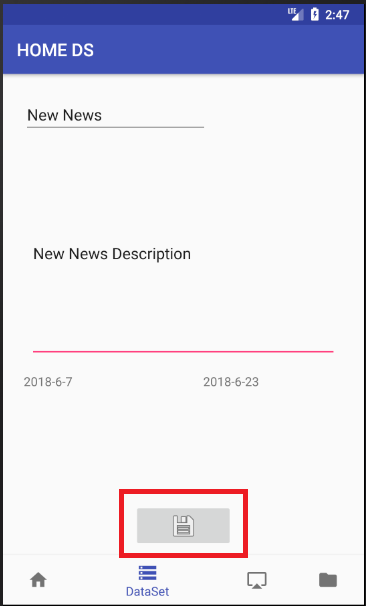
\includegraphics[width=1.0\textwidth]{images/06_AndroidApp/06_EditNewsSaveButton}
\caption{Markierte Liste mit Layouts und Navigationstab}
\label{fig:mediaNav}
\end{figure}
\\
Die Liste zeigt alle am Server befindlichen Layouts durch klicken einer der Listenelemente navigiert die Applikation zu einer Detailansicht des Layouts.
\\
\begin{figure}[H]
\centering
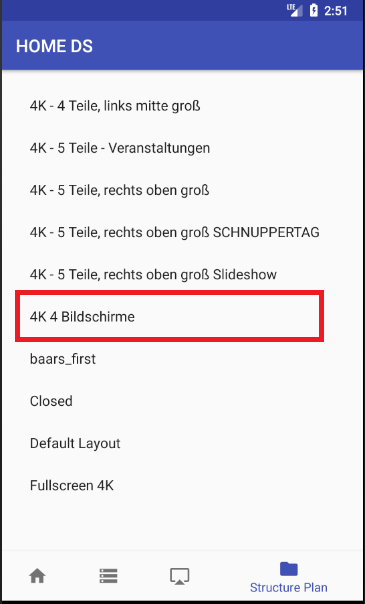
\includegraphics[width=1.0\textwidth]{images/06_AndroidApp/06_StructureNavigationToDetail}
\caption{Markiertes Element um auf die Detailansicht zu gelangen}
\label{fig:mediaNav}
\end{figure}
\\
Die Detailansicht eines Layouts zeigt die Grunddaten eines Layouts wie zum Beispiel die ID oder die Besitzer ID. Des weiteren werden alle unterelemente beispielsweise Widget's angezeigt. Dargestellt wird der JSON-String des Layouts.
\\
\begin{figure}[H]
\centering
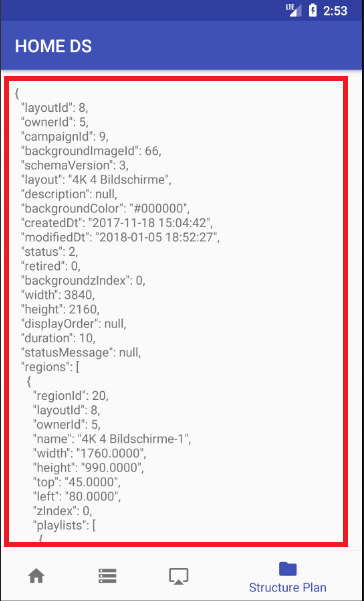
\includegraphics[width=1.0\textwidth]{images/06_AndroidApp/06_StructureDetail}
\caption{Markierte Details des Layouts}
\label{fig:mediaNav}
\end{figure}
\\
\section{MainBottomNavigationActivity und OverviewFragment}
\subsection{MainBottomNavigationActivity}
\\
\begin{figure}[H]
\centering
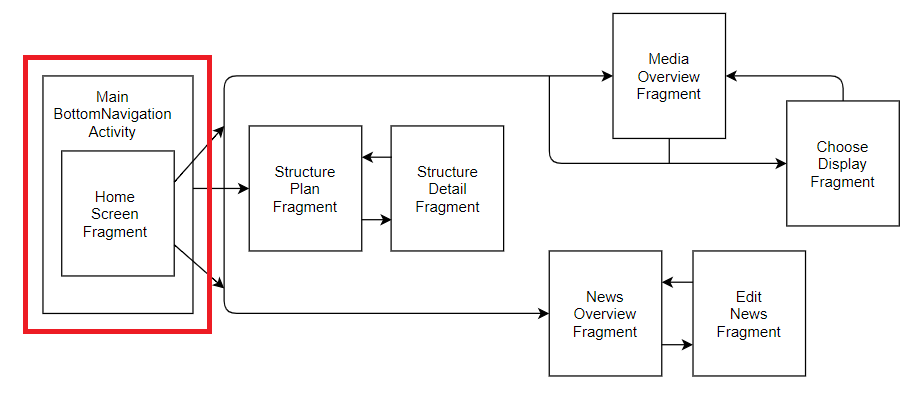
\includegraphics[width=1.0\textwidth]{images/06_AndroidApp/06_AndroidArchMainBottomNavigationActivity}
\caption{Stellung des MainBottomNavigationFragemt in der Android Applikation}
\label{fig:mediaNav}
\end{figure}
\\
Die ''MainBottomNavigationActivity'' ist die Einzige ''Activity'' die in der Android Applikation benötigt wird. Hauptaufgabe der ''MainBottomNavigationActivity'' ist es, zwischen den einzelnen ''Fragments'' zu navigieren. Enthalten sind dazu jene Methoden, welche mit dem ''SupportFragmentManager'' die einzelnen Fragments im ''container\_main'' austauschen. Der ''container\_main'' ist ein ''ConstraintLayout'' welches in der zur ''MainActivity'' gehörenden Layout Ressource ''activity\_main.xml'' mit der Identifikationsnummer ''container\_main'' und  belegt wurde. Zudem wird die Klasse durch das Interface ''AppCompatActivity'' erweitert und implementiert die ''OnFragmentInteractionListener'' der Fragmente die in der Applikation verwendet werden. 
\
Im unteren Teil der ''Activity'' befindet sich eine Navigationsleiste. Diese ist zuständig für das wechseln zwischen den einzelnen Fragmenten mit folgenden Navigationspunkten: 

\begin{itemize}
	\item {\em Home:} Jener Menüpunkt der die Startseite der Applikation beinhaltet.
	\item {\em DataSet:} Ist zuständig für die Verwaltung der ''DataSets''.
	\item{\em Medium abspielen:} Beinhaltet die Fragmente die benötigt werden um Medien auf der gewünschten anzeige abzuspielen.
	\item {\em Strukturplan:} Bietet eine Übersicht über die Struktur der am Server liegenden Layouts.
\end{itemize}
\subsubsection{onCreate}
Hier wird die ''MainBottomNavigationActivity'' als ''ContentView'' gesetzt, zudem wird mittels ''SupportFragmentManager'' das ''HomeScreenFragment'' dem ''container\_main'' zugewiesen und angezeigt. Das Feld Display wird neu instantiiert. Die statische Variable ''instance'', vom Datentyp ''MainBottomNavigationActivity'', wird auf die aktuelle Instanz der Klasse zugewiesen. Die ''BottomNavigationBar wird mit werten belegt und ein ''OnNavigationItemSelectedListener'' gesetzt um durch die Applikation navigieren zu können.
\begin{lstlisting}[language=Java, caption={}
setContentView(R.layout.
	activity_main_bottom_navigation);
mainActivityBottomNavigation = this;
openHomeScreenFragment();
display = new Display();
 
navbar = findViewById(R.id.navigation_bar);
navbar.setOnNavigationItemSelectedListener(
	new BottomNavigationView.
   	OnNavigationItemSelectedListener() {
    	@Override
     	public boolean onNavigationItemSelected(
     				@NonNull MenuItem item) {
     		item.setChecked(true);
        	switch (item.getItemId()) {
        		case R.id.editDatasetNavBar:
            		openNewsOverview();
                	break;
            	case R.id.playMediaNavBar:
                	if (display.getDisplay() == null){
                	openChooseDisplayFragment();
                	}else {
                	openMediaOverviewFragment();
                	}
                	break;
            	case R.id.homeScreenNavBar:
                	openHomeScreenFragment();
                	break;
            	case R.id.structurePlanNavBar:
                	openStructurePlanFragment();
                	break;
                	}
          	return false;
        }
	});
\end{lstlisting}	
\subsubsection{getInstance}
 Ist der ''Getter'' für die statische Variable ''instance'' und übergibt die aktuelle Instanz der Klasse.
\begin{lstlisting}[language=Java, caption={}
public static MainActivityBottomNavigation
	 getInstance() {
     return mainActivityBottomNavigation;
}
\end{lstlisting}
\subsubsection{Fragment-Austausch-Methoden}
 Sind jene Methoden die für das Austauschen der einzelnen ''Fragments'' im ''container\_main'' zuständig sind. Dies geschieht mittels ''SupportFragmentManager'' welcher immer die ''Fragments'' im ''container\_main'' anzeigt und dem ''BackStack'', welcher für die Rückwerts Navigation (mittels retour Knopf des Mobilen Endgerätes) in der Applikation zuständig ist,  hinzufügt. Manche Methoden übergeben zudem noch ein ''Bundle'' an das erstellte ''Fragment'', welches Objekte enthält die in nächsten ''Fragment'' benötigt werden. Erkennungsmerkmal dieser Methoden ist das englische Verb ''open'' am beginn des Methodennamens. Als Namensbeispiel hierfür wird die Methode ''openNewsEditFragment'' herangezogen.
\begin{lstlisting}[language=Java, caption={}
public void openEditNewsFragment(DataSetDataField news) {
Bundle bundle = new Bundle();
bundle.putSerializable("data", news);
NewsEditFragment newsEditFragment =
    new NewsEditFragment();
newsEditFragment.setArguments(bundle);
FragmentManager fm = getSupportFragmentManager();
fm.beginTransaction().replace(
    R.id.container_display, 	
    newsEditFragment,"actEdit")
    .addToBackStack("actEdit").commit();
}
\end{lstlisting}
\subsection{HomeScreenFragment}
\\
\begin{figure}[H]
\centering
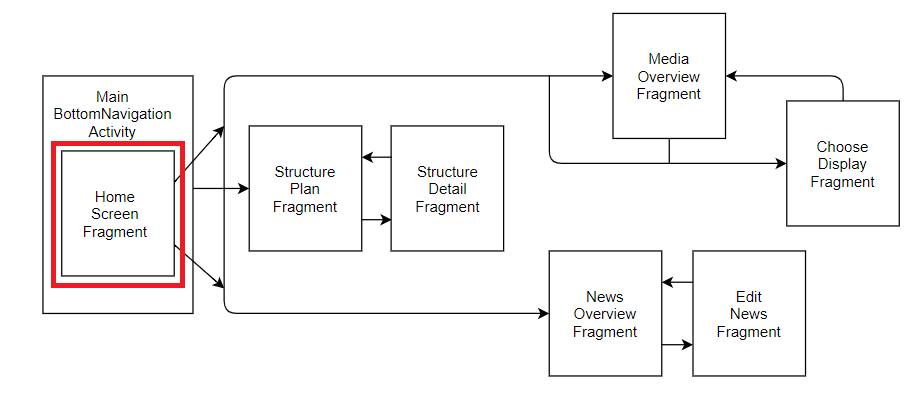
\includegraphics[width=1.0\textwidth]{images/06_AndroidApp/06_AndroidArchHomeScreen}
\caption{Stellung des HomeScreenFragmnet in der Android Applikation}
\label{fig:mediaNav}
\end{figure}
\\
Der Einstiegspunkt der Applikation ist das ''HomeScreenFragment''. Es zeigt den Serverstatus an, dieser wird über einen ''REST-Request'' vom Java-EE-Server abgefragt. Den Hauptanteil des Fragments bilden die beiden Navigations-Buttons ''Median abspielen'' und ''Eilmeldungen anzeigen''. Durch klicken dieser Buttons öffnen sich die dazugehörigen Fragmente ''NewsOverviewFragment'' und ''MediaOverviewFragment''.
\\
Die Layout Ressource des ''HomeScreenFragment'' enthält zwei Buttons und ein ''ConstaintLayout''. Dieses ''ConstraintLayout'' beinhaltet wiederum eine ''TextView'' und zwei ''ImageViews''. In der ''onCreate'' Methode des Fragments werden als erstes die Anzeigeelemente neu deklarierten Variablen zugewiesen und im ''ConstraintLayout'' wird der Serverstatus auf View standardmäßig als Offline angezeigt und die Buttons deaktiviert.
\begin{lstlisting}[language=Java, caption={}
Button btPlayMedia = v.findViewById(R.id.btPlayMedia);
Button btShowNews = v.findViewById(R.id.btShowNews);

btPlayMedia.setEnabled(false);
btShowNews.setEnabled(false);
    
ImageView ivUp = v.findViewById(R.id.ivServerUp);
ivUp.setVisibility(View.INVISIBLE);
    
ImageView ivDown = v.findViewById(R.id.ivServerDown);    
ivDown.setVisibility(View.VISIBLE);
    
ConstraintLayout clServerStatus = 
    v.findViewById(R.id.cl_serverStatus);
clServerStatus.setBackgroundColor(
    ContextCompat.getColor(
    this.getContext(), R.color.serverDown));
}
\end{lstlisting}
Im folgenden Schritt wird über einen ''GET-Request'' die Uhrzeit des XIBO-Servers über den Java-EE-Server abgefragt. Wird eine Uhrzeit vom erhalten, so wird im ''ConstraintLayout'' des Server Status auf online gesetzt und das dazugehörige Bild angezeigt und die Buttons werden freigegeben. Erhält man keine Antwort bleibt die Anzeige unverändert.

\begin{lstlisting}[language=Java, caption={}
rh.executeRequest(RequestTypeEnum.GET, null,
	MainActivityBottomNavigation.getInstance()
	.url + "/status/", () -> {   
    MainActivityBottomNavigation.getInstance()
    .runOnUiThread(() -> {
      	if (rh.getResponseCode() == 200) {
        	
           	ivUp.setVisibility(View.VISIBLE);
            ivDown.setVisibility(View.INVISIBLE);
                
            clServerStatus.setBackgroundColor(
           	ContextCompat.getColor(this.getContext(),
           	R.color.serverUp));
                	
            btPlayMedia.setEnabled(true);
            btShowNews.setEnabled(true);
                    
         }else {
         	ivDown.setVisibility(View.VISIBLE);
                    
            clServerStatus.setBackgroundColor(
            	ContextCompat.getColor(this.getContext(),
                R.color.serverDown));
            }
    });
});
\end{lstlisting}
Um die Navigation über die erstellten Buttons zu ermöglichen wird ein ''OnClickListener'' Implementiert.
\begin{lstlisting}[language=Java, caption={}
btPlayMedia.setOnClickListener(
	new View.OnClickListener() {
            
    	@Override
        public void onClick(View view) {
            MainActivityBottomNavigation.
            getInstance().navbar
            .setSelectedItemId(R.id.playMediaNavBar);
        }
     });
\end{lstlisting}
\section{DataSet Verwaltung}
\\
\begin{figure}[H]
\centering
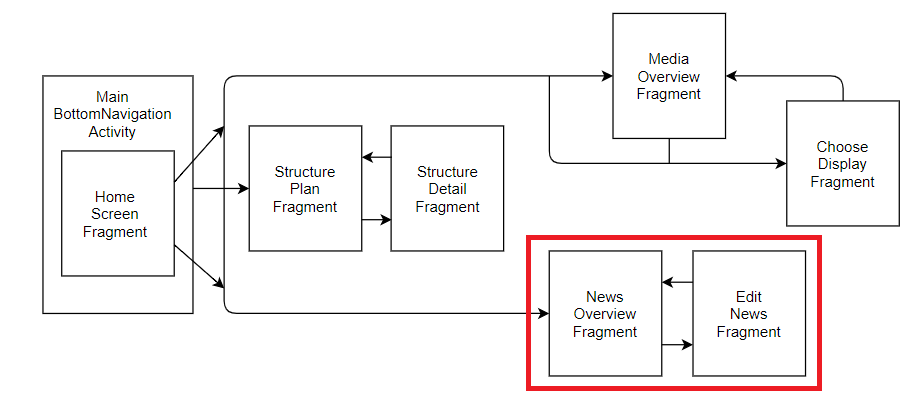
\includegraphics[width=1.0\textwidth]{images/06_AndroidApp/06_AndroidArchShowNews}
\caption{Stellung der DataSet Verwaltung in der Android Applikation}
\label{fig:mediaNav}
\end{figure}
\\
Die beiden Fragmente  ''NewsOverviewFragment'' und ''NewsEditFragment'' sind für die Verwaltung der ''DataSets'' zuständig. Im Fragment ''NewsOverviewFragment'' wird eine Übersicht über alle vorhandenen ''DataSets'' gegeben. Das ''NewsEditFragment'' Fragment wird verwendet um vorhandene ''DataSets'' zu bearbeiten oder neue ''DataSets'' zu erstellen. 
\subsubsection{NewsOverviewFragment}
Dieses Fragment zeigt alle aktiven ''DataSets'' an, diese werden vom Server bereitgestellt und per ''REST-Request'' abgefragt. Über einen ''FloatingActionButton'' kann ein neues ''DataSet'' erstellt werden. Durch klicken auf eines der Listen Elemente, öffnet sich eine Detailansicht in der das Bearbeiten, eines des ''DataSets'' möglich ist.
\\
\begin{figure}[H]
\centering
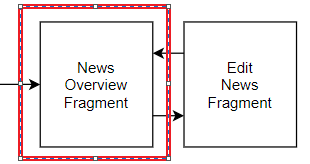
\includegraphics[width=1.0\textwidth]{images/06_AndroidApp/06_NewsOverviewStellung}
\caption{Stellung des NewsOverViewFragment in der Android Applikation}
\label{fig:mediaNav}
\end{figure}
\\
Die Layout Ressource des Fragments, ''fragment\_news\_overview.xml'' enthält eine ''RecyclerView'' und einen ''FloatingActionButton''. Die Logik der Anzeige ist in der Java Klasse ''NewsOverviewFragment'' implementiert. Die meisten Methoden dieser Klasse werden generisch beim Erstellen eines Fragments erzeugt. Die einzige Methode die überschrieben wurde ist die Methode ''onCreateView''. Beim Ausführen dieser Methode wird zuerst eine ''View'' erstellt welche das ''fragment\_news\_overview'' Layout zugewiesen bekommt. Anschließend wird eine ''RecyclerView'' und ein ''FlaootingActionButton'' erstellt und den zugehörigen Anzeige Elementen zugewiesen.
\begin{lstlisting}[language=Java, caption={}
View v = inflater.inflate(
	R.layout.fragment_news_overview, container, false);
RecyclerView rv = v.findViewById(R.id.rvNews);

FloatingActionButton fabAddNews = 
    v.findViewById(R.id.fabAddNews);

\end{lstlisting}
 Der ''FlaootingActionButton'' erhält einen ''OnClickListener'' über diesen wird in der ''MainActivity'' eine Methode aufgerufen die ein neues ''NewsEditFragment'' anzeigt, um ein neues ''DataSet'' zu erstellen. 
 \begin{lstlisting}[language=Java, caption={}
fabAddNews.setOnClickListener(
	new View.OnClickListener() {
        @Override
        public void onClick(View view) {
            MainActivityBottomNavigation.
            getInstance().
            openEditNewsFragment(
            new DataSetDataField());
        }
    });
\end{lstlisting}
Um in der ''RecyclerView'' Elemente anzeigen zu können werden diese über einen REST-Request an den Server abgefragt und der ''RecyclerView'' übergeben.
\begin{lstlisting}[language=Java, caption={}
rh.executeRequest(RequestTypeEnum.GET, null,
	MainActivityBottomNavigation
	.getInstance().url 
	+ "/datasetdatafield/", () -> {

        MainActivityBottomNavigation.getInstance()
        .runOnUiThread(() -> {
            //Belegung der angezeigten Elemente
        });
    });
\end{lstlisting}
\subsubsection{NewsEditFragment}
\\
\begin{figure}[H]
\centering
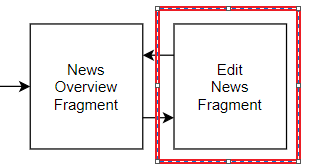
\includegraphics[width=1.0\textwidth]{images\06_AndroidApp\06_NewsEditStellung}
\caption{Stellung des NewsEditFragment in der Android Applikation}
\label{fig:mediaNav}
\end{figure}
\\
Das Fragment zeigt alle Details eines ''DataSets'' an und bietet die Möglichkeit die Detailinformationen bearbeiten zu können. Ebenso wird dieses Fragment dazu verwendet, ein neues ''DataSet'' zu erstellen, dazu wird das Fragment mit Hinweisen auf die Eingabeoptionen erstellt. Über einen Button können die eingegeben Felder an den ''Java-EE-Server'' übermittelt werden. Eingabe Felder:
\begin{itemize}
	\item {\em Titel:} Das Feld ''Titel'' beinhaltet die Überschrift der anzuzeigenden Information.
	\item {\em Beschreibung:} Hier wird der eigentliche Informationstext eingefügt.
	\item{\em Datum-Von-Bis:} Diese Felder werden über ein ''DatePickerDialog'' befüllt, welcher einen Kalender öffnet und zeigen an in welchen Zeitraum das ''DataSet'' angezeigt wird. 
	\item {\em Uhrzeit-Von-Bis:} Die anzeige Elemente geben Auskunft über die Zeitspanne in der das ''DataSet'' an den einzelnen Tagen angezeigt wird. Das Feld kann mittels ''TimePickerDialog'' befüllt werden.		
\end{itemize}
Anzeige Ressourcen für dieses Fragment werden in der Datei ''fragment\_news\_edit.xml'' bereitgestellt. Diese enthält die benötigten Tags, um die im oberen Teil beschrieben Eingabefelder zur Verfügung zu stellen. Die Verwendung und Belegung dieser Felder wird in der Klasse ''NewsEditFragment'' implementiert. Auch in dieser Klasse wurde nur die Methode ''onCreateView'' mit Quellcode versehen. Zu Beginn wird der deklarierten ''View'' die ''fragment\_news\_edit.xml'' als Ressource zugewiesen. Um Daten aus dem ''NewsOverviewFragment'' zu empfangen wird ein ''Bundle'' befüllt. Wenn das befüllte ''Bundle'' Informationen beinhaltet, dann wird die Funktion ''setArguments'' der Basisklasse Fragment(android.support.v4.app.Fragment) mit dem Parameter ''bundle'' aufgerufen, um das Feld ''mArguments'' der Basisklasse Fragment mit Daten zu versehen(Vererbung). Die zuvor deklarierten Variablen (benötigte ''Views'') werden jetzt initialisiert.
\begin{lstlisting}[language=Java, caption={}
Bundle bundle = getArguments();
Log.d("BUNDLDATA", String.valueOf(bundle));
if (bundle != null){
    this.setArguments(bundle);
    }
            
DataSetDataField news =
 	(DataSetDataField) bundle.getSerializable("data");
ImageButton ibSaveNews =
  	v.findViewById(R.id.ibSaveNews);
        
title = v.findViewById(R.id.etTitle);
description = v.findViewById(R.id.etDescription);

title.setText(news.getTitle());
description.setText(news.getValue());

tvTimeFrom = v.findViewById(R.id.tvTimeFrom);
tvTimeTo = v.findViewById(R.id.tvTimeTo);
\end{lstlisting}

Das Fragment hat zwei verschiedene Vorgehensweisen. Zum einen werden, sollte ein ''DataSet'' in Form eines ''Bundels'' übergeben werden, die Anzeigeelemente mit den übergebenen Werten befüllt. Andernfalls werden die Felder mit keinen Werten versehen, es werdend Hinweise auf die Eingabeoptionen im aktuellen Fragment angezeigt.

\begin{lstlisting}[language=Java, caption={}
if (news.getToDate() != null 
		&& news.getFromDate() != null) {
    tvTimeFrom.setText(news.getFromDate().toString());
    tvTimeTo.setText(news.getToDate().toString());
    dateTo = news.getToDate();
    dateFrom = news.getFromDate();
}   
\end{lstlisting}

Die benötigten ''onClickListener'' für die Datums und Uhrzeit eingaben werden im Anschluss implementiert und mittels ''DatePickerDialog'' beziehungsweise ''TimePickerDialog'' mit Daten versehen. 
\begin{lstlisting}[language=Java, caption={}
tvTimeTo.setOnClickListener(new View.OnClickListener() {
	@Override
    public void onClick(View view) {
    	final Calendar c = Calendar.getInstance();
        year = c.get(Calendar.YEAR);
        month = c.get(Calendar.MONTH);
        day = c.get(Calendar.DAY_OF_MONTH);

        DatePickerDialog datePickerDialog = 
        	new DatePickerDialog(
            MainActivityBottomNavigation.getInstance()
            , new DatePickerDialog.OnDateSetListener() {
            	@Override
                public void onDateSet(
                  		DatePicker datePicker,
                   		int year, int month, int day) {
                	tvTimeTo.setText(year + "-" 
                        			+ (month + 1)
                        			+ "-" + day);
                    dateTo = LocalDate.
                    	of(year, month, day);
                }
            }, year, month, day);
            datePickerDialog.show();
        }
    });
\end{lstlisting}

Durch Drücken des Buttons(Speicher Button) wird ein Event ausgelöst. Dieses Event kann zwei verschiedene Ausgänge haben: Wenn das im Event erhaltene ''Bundle'' eine ''ID'' besitzt, lässt sich daraus eindeutig schließen, ob es sich hierbei um ein Dataset handelt, das vom User erstellt wurde, oder um eines, das bereits zuvor am Java-EE-Server vorhanden war, indem man überpfrüft, ob die im Bundle enthaltene Information ''ID'' den Wert null hat, oder nicht. Falls dies nämlich der Fall ist, sind es eindeutig vom Benutzer eingegebene Daten. Somit muss deswegen am Server anschließend ein ''POST-Request'' durchgeführt werden, um die neu erstellten Informationen zu senden.
Wenn es ein vom Java-EE-Server erhaltenes ''DataSet'' ist, wird stattdessen ein ''PUT-Request'' durchgeführt, der die veränderten Daten übermittelt. 
\begin{lstlisting}[language=Java, caption={}
if (news.getId() != null && news.getDataSetId() 
		!= null && news.getDataRowId() != null) {
	params.put("id", news.getId().toString());
    params.put("dataSetId", news.getDataSetId().toString());
    params.put("dataRowId", news.getDataRowId().toString());
   } 
       
if (news.getId() == null) {
    Long n = -1L;
    params.put("dataRowId", n.toString());
    rh.executeRequest(RequestTypeEnum.POST, params,
       	MainActivityBottomNavigation
        .getInstance().url + "/datasetdatafield/save/",
         () -> {
          //Toast ausgabe
        });
}  else {
    rh.executeRequest(RequestTypeEnum.PUT, params,
        MainActivityBottomNavigation
        .getInstance().url + "/datasetdatafield/edit/",
       	() -> { 
          //Toast ausgabe
        });                 
    }
\end{lstlisting} 
\section{Mediaplayer}
\\
\begin{figure}[H]
\centering
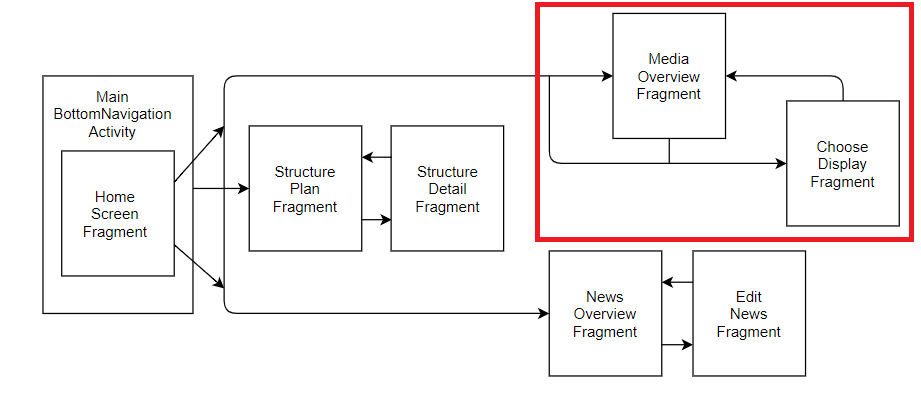
\includegraphics[width=1.0\textwidth]{images\06_AndroidApp\06_AndroidArchPlayMedia}
\caption{Stellung der Media Navigation in der Android Applikation}
\label{fig:mediaNav}
\end{figure}
\\
Um auf einer gewünschten Anzeige ein, sich auf dem Server befindliches, Medium abzuspielen wurden die beiden Fragments ''MediaOverViewFragment'' und ''ChooseDisplayFragment'' implementiert. Das gewünschte Medium wird auf dem ausgewählten Display sofort Abgespielt. Ist noch kein Display ausgewählt wird man zuerst auf das ''ChooseDisplayFragment''gelitet um einen anzeige Display zu wählen.
\subsubsection{MediaOverviewFragment}
Im diesem Fragment werden alle Medien angezeigt, die sich am XIBO-Server in der Bibliothek befinden und mit dem Richtigen Tag markiert sind. Eine Sortierung der Liste ist über ein ''Spinner'' Element möglich. Des weiteren wird im rechten oberen teil des Fragments der Display angezeigt auf dem das gewählte Medium abgespielt werden soll. Eine Auswahl des Displays ist über Navigation zum ''ChooseDisplayFragment'' möglich, dieses wird über den Button ''Auswählen'' geöffnet. Hat der Benutzer noch keinen keinen Display ausgewählt wird er zuerst auf das ''ChooseDisplayFragment'' weitergeleitet.
\\
\begin{mediaNav}
\centering
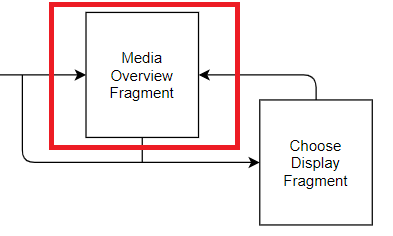
\includegraphics[width=1.0\textwidth]{images\06_AndroidApp\06_MediaOverViewStellung}
\caption{Stellung des MediaOverViewFragment in der Android Applikation}
\label{fig:mediaNav}
\end{mediaNav}
\\
Durch die Ressource Datei ''fragment\_media\_overview.xml'' können die Elemente in der View angezeigt werden. Dieses Layout beinhaltet neben einer ''RecyclerView'' zur Darstellung der abzuspielenden Medien, zwei Buttons eine TextView und einen Spinner zur Sortierung der angezeigten Liste. Einstiegspunkt der Methode ''onCreateView'' ist die zuweisung der Layout Ressource. Weiters werden die in der Klasse deklarierten Variablem mit den Anzeigeelementen verknüpft. Die TextView wird im Anschluss mit dem Namen des, für die Wiedergabe gewählten, Displays belegt.
\begin{lstlisting}[language=Java, caption={}
View v = inflater.inflate(
	R.layout.fragment_media_overview, container, false);
rvMedia = v.findViewById(R.id.rvMedia);
medias = new LinkedList<>();
spTagChoise = v.findViewById(R.id.spTagChoise);
btCooseDisplay = v.findViewById(R.id.btChooseDisplay);
tvDisplayToPlay = v.findViewById(R.id.tvDisplayToPlay);
tvDisplayToPlay.setText(
	MainActivityBottomNavigation.getInstance()
	.getDisplay().getDisplay()); 
\end{lstlisting}
Um die Liste der Medien nach nach belieben zu sortieren wird ein ArrayAdapter initialisiert. Diesem werden die Ressourcen ''tag\_array'', beinhaltet eine Liste mit Sortiermöglichkeiten für die angezeigten Medien, und ''simple\_spinner\_item'' um das Design für die angezeigten ''Spinner'' Elemente, übergeben. Es erfolgt eine Zuweisung des Adapters an das Spinner Element. Um die Sortierung der Medien Liste zu realisieren wird ein ''OnItemSelectedListener'' implementiert der die Medien gefiltert nach ausgewähltem Tag anzeigt. Um zu beginn alle Inhalte anzuzeigen wird dem Spinner das erste Element des ''tag\_array'' als Standardsortierung zugewiesen.
\begin{lstlisting}[language=Java, caption={}
ArrayAdapter<CharSequence> tagAdapter =
	ArrayAdapter.createFromResource(
    MainActivityBottomNavigation.getInstance()
    .getApplicationContext(), R.array.tag_array,
    android.R.layout.simple_spinner_item);
        
tagAdapter.setDropDownViewResource(
	android.R.layout.simple_spinner_dropdown_item);
    	
spTagChoise.setAdapter(tagAdapter);
spTagChoise.setOnItemSelectedListener(
	new AdapterView.OnItemSelectedListener() {
        @Override
        public void onItemSelected(AdapterView<?> adapterView,
        						 View view, int i, long l) {
            mediaTag = adapterView
            	.getItemAtPosition(i).toString();
            setRecyclerView(mediaTag,rvMedia);
        }
        @Override
        public void onNothingSelected(AdapterView<?> adapterView) {
            spTagChoise.setSelection(0);
            mediaTag = adapterView.getItemAtPosition(0).toString();
            setRecyclerView(mediaTag,rvMedia);
        }
    });
spTagChoise.setSelection(0);

mediaTag = spTagChoise.getItemAtPosition(0).toString();
\end{lstlisting}
Um zwischen den Einzelnen Displays zu wählen wird dem ''Auswählen'' Button ein ''onClickListener'' zugewiesen welcher die Navigation zum ''ChooseDisplayFragment'' einleitet.

\begin{lstlisting}[language=Java, caption={}
btCooseDisplay.setOnClickListener(new View.OnClickListener() {
   	@Override
    public void onClick(View view) {
    	MainActivityBottomNavigation
    	.getInstance().openChooseDisplayFragment();
      	
        tvDisplayToPlay.setText(
        	MainActivityBottomNavigation.getInstance()
        	.getDisplay().getDisplay());
        }
    });
\end{lstlisting}

Des weiteren wurde die Methode ''setRecyclerView'' erstellt um die Daten nach Tag sortiert vom Server mittels ''GET-Request'' zu erhalten und diese auf der View anzeigen zu können.


\begin{lstlisting}[language=Java, caption={}
HashMap<String, String> params = new HashMap<>();
params.put("start", "1");
params.put("length", "10");
params.put("tags", mediaTag);
        
rh.executeRequest(RequestTypeEnum.GET, params, 										MainActivityBottomNavigation.getInstance()
    .url + "/media/", () -> {
    	MainActivityBottomNavigation.getInstance()
    	.runOnUiThread(() -> {
			//Belegung der angezeigten Elemente            
		});
\end{lstlisting}
\subsubsection{ChooseDisplayFragment}
Die Auswahl des Bildschirmes auf dem das Medium angezeigt werden soll erfolgt über dieses Fragment. Dazu werden die verfügbaren Displays vom Java-EE-Server abgefragt und in einer Liste angezeigt. Durch klicken auf den ''Aüswählen'' Button in einem der in der Liste angezeigten Display Elementen, wird dieser Display ausgewählt und Medien werden dann auf diesem Abgespielt. 
\\
\begin{figure}[H]
\centering
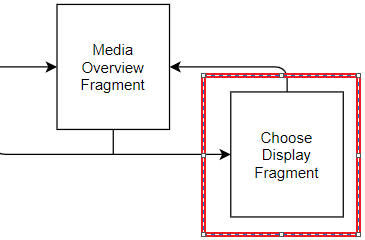
\includegraphics[width=1.0\textwidth]{images\06_AndroidApp\06_ChooseDisplayStellung}
\caption{Stellung des ChooseDisplayFragment in der Android Applikation}
\label{fig:mediaNav}
\end{figure}
\\
Die RecyclerView Ressource um die zu wählenden Displays anzuzeigen ist in der Datei ''fragment\_choose\_display.xml'' angelegt. Zuweisen der Layout ressource auf die aktuelle View, initialisieren der Klassen Attribute und aufrufen der Methode ''getDisplays'' sind die einzigen Schritte der ''onCreateView'' Funktion.''getDisplays'' ist jene Methode die alle Displays die mit dem XIBO-Server verbunden sind per ''GET-Request'' abfragt beziehungsweise aufbereitet und der RecyclerView übergibt um diese auf der View anzuzeigen. 
\begin{lstlisting}[language=Java, caption={}
rh.executeRequest(RequestTypeEnum.GET, null, 				^						MainActivityBottomNavigation.getInstance().
	url + "/display/", () -> {
		//Belegung der angezeigten Elemente
	});
\end{lstlisting}
\section{Strukturplan}
\\
\begin{figure}[H]
\centering
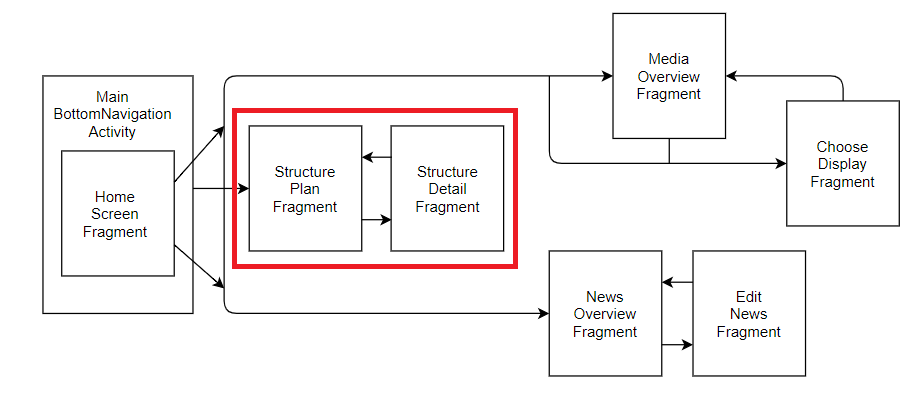
\includegraphics[width=1.0\textwidth]{images\06_AndroidApp\06_AndroidArchStructureCrawler}
\caption{Stellung der Strukturverwaltung in der Android Applikation}
\label{fig:mediaNav}
\end{figure}
\\	
Die am XIBO-Server liegenden Layouts werden in der Andoid Applikation formatiert als ''JSON-Sting'' angezeigt. Damit ist gewährleistet, dass der App-Benutzer eine Übersicht über die Struktur der einzelnen Layouts und deren Unterelemente zur Verfügung hat.
\subsubsection{StructurePlanFragment}
Dieses Fragment zeigt eine Übersicht der einzelnen Layouts in Form einer Liste an. Durch klicken der einzelnen Listen Elemente navigiert die Applikation zu einer Detailansicht über das gewählte Layout.
\\
\begin{figure}[H]
\centering
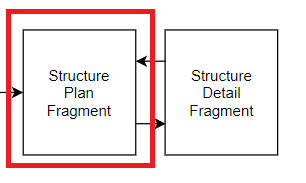
\includegraphics[width=1.0\textwidth]{images\06_AndroidApp\06_StructurePlanStellung}
\caption{Stellung des StructurePlanFragment in der Android Applikation}
\label{fig:mediaNav}
\end{figure}
\\	
Die Ressource zur gestaltung der Anzeige beinhaltet eine ''RecyclerView'' und heißt ''fragment\_structure\_plan.xml''. Zu beginn der ''onCreateView'' Methode wird zuerst eine ''View'' erstellt welche das ''fragment\_structure\_plan.xml'' Layout zugewiesen bekommt. Die ''RecyclerView'' wird anschließend initialisiert und über einen ''GET-Request'', dessen Response die einzelnen Layouts und deren Unterstrukturen,des Xibo-Servers in form eines JSON-Strings übermittelt, befüllt. Somit ist auf der Anzeige eine Liste mit auswählbaren Layouts vorhanden über die zu einer Detailansicht navigiert werden kann. 
\begin{lstlisting}[language=Java, caption={}
RecyclerView rvStructurePlan = v.findViewById(R.id.rvStructurePlan);
HashMap<String,String> params = new HashMap<>();
params.put("layoutId","-1");
    
rh.executeRequest(RequestTypeEnum.GET,params
	,MainActivityBottomNavigation.getInstance()
	.url + "/crawler/", ()->{
		//Belegung der angezeigten Elemente
		}
\end{lstlisting}

\subsubsection{StructureDetailFragment}
Ein Layout wird in diesem Fragment in Form eines ''JSON-Strings'' mit allen dazugehörigen Unterelementen angezeigt. Wichtig hierbei ist es den Angezeigten ''JSON-String'' richtig zu formatieren um die Übersichtlichkeit bei zu behalten.
\\
\begin{figure}[H]
\centering
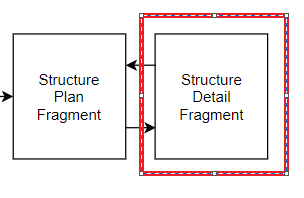
\includegraphics[width=1.0\textwidth]{images\06_AndroidApp\06_StructureDetailStellung}
\caption{Stellung des StructureDetaiFragment in der Android Applikation}
\label{fig:mediaNav}
\end{figure}
\\
In der Ressource Datei ''fragment\_structure\_detail.xml'' befindet sich eine ''TextView'' als einziges Element. Die ''onCreateView'' Methode der Klasse ''StructureDetailFragment'', wird nach zuweisen der Layout Ressource der Struktur beschreibende ''JSON-String'' aus dem ''Bundle'' gelesen, dies geschieht über die Methode ''setArguemnts'' der Basisklasse Fragment und deren Feld ''mArguments'', und dem Anzeigefeld zugewiesen. Anschließend wird dem Fragment noch die fähigkeit gegeben sich Scrollen zu lassen und die View wird zurückgegeben. 
\begin{lstlisting}[language=Java, caption={}
View v = inflater.inflate(
	R.layout.fragment_structure_detail, container, false);
Bundle bundle = this.getArguments();
TextView tvStructureDetailString = 													v.findViewById(R.id.tvStructureDetailString);
    
String detail = bundle.getString("actStructure");
    
tvStructureDetailString.setText(detail.toString());    tvStructureDetailString.setMovementMethod(
    new ScrollingMovementMethod());
\end{lstlisting}
\section{Request-Helper}
Um in weiterer Folge die Anfragen an den Java-EE-Server einfach und einheitlich durchzuführen gibt es die Klasse ''RequestHelper'' . In dieser Klasse gibt es neben den beiden Parametern ''responseBody'' und ''responseCode'', welche zur Fehlerausgabe und zum Erhalt der Daten aus der Anfrage vorhanden sind, die Methode ''executeRequest''. Diese übernimmt die Hauptaufgabe der Klasse und führt die Anfragen an das Signage System durch. Werden Daten als Antwort der anfrage erwartet so kann die Methode mit ''Callback'' Parameter aufgerufen werden, ist dies nicht der Fall so gibt es die Möglichkeit diese Methode ohne ''Callback'' aufzurufen, dabei wird dieser Parameter mit dem Wert null überschrieben.
\\
Die Parameter dieser Methode lauten wie folgt:
\\
\begin{itemize}
	\item {\em RequestTypeEnum:} Der Parameter vom Typ Enum wird genutzt um Herauszufinden welche Http Anfrage vorliegt. Mögliche Werte sind hierbei GET, POST, PUT und DELETE.
	
	\item {\em Params:} Hier liegt eine HashMap vor, die als Key-Value Paare alle benötigten Parameter für den RequestBody beinhaltet. Beispielsweise: ''LayoutID'':''78'', hierbei ist ''LayoutID'' der Key und ''78'' das Value.
		
	\item {\em Url:} Beinhaltet die URL unter der die Anfrage erreichbar ist. 
	
	\item {\em Callback:} Dieser Parameter wird benötigt, um auf eine Antwort des ausgeführten ''REST-Request'' zu warten. Wird ein ''Response'' erhalten und die Daten werden in dem angezeigten Fragment benötigt, können diese über eine ''Lamda-Expression'' in die gewünschten Anzeigeelemente eingefügt werden. 
\end{itemize}
Zu Beginn der Methode wird anhand des Parameters RequestTypeEnum unterschieden, um welche Http Anfrage es sich handelt. Wird GET oder DELETE geliefert wird durch die HashMap iteriert und die einzelnen Key-Value Paare als QeryParameter in der URL einfügt.
Beispielsweise:''<URL>/layout?layoutID=78'' .
\begin{lstlisting}[language=Java, caption={}
if (params != null && params.size() > 0) {
    Iterator it = params.entrySet().iterator();
    while (it.hasNext()) {
     	Map.Entry p = (Map.Entry) it.next();
	    urlBuilder.addQueryParameter(
	      	p.getKey().toString(), p.getValue().toString());
        }
    }
\end{lstlisting}
Handelt es sich um eine POST oder PUT Anfrage so werden die Key-Value Paare im Body mitgegeben und im Format "application/x-www-form-urlencoded" codiert.
\begin{lstlisting}[language=Java, caption={}
String stringbody = "{";
if (params != null && params.size() > 0) {
  	Iterator it = params.entrySet().iterator();
    while (it.hasNext()) {
       	Map.Entry p = (Map.Entry) it.next();
        stringbody += "\"" 
        + p.getKey().toString() 
        + "\"" + ":" + "\"" 
        + p.getValue().toString() 
        + "\"" + ",";
        }
    }
stringbody = stringbody.substring(
  	0, stringbody.length() - 1);
stringbody += "}";
body = RequestBody.create(
MediaType.parse("application/json")
       			, stringbody);
\end{lstlisting}
Anschließend wird die URL mittels HttpUrl.Builder erstellt und ausgegeben. 
Des Weiteren wird per Switch-Case dem Request die richtige Art der Anfrage zugewiesen und danach die URL übergeben. 
\begin{lstlisting}[language=Java, caption={}
URL finalUrl = urlBuilder.build().url();
    Log.i(LOGTAG, "FinalUrl: " + finalUrl.toString());
    Request.Builder rb = new Request.Builder();
    switch (executeType) {
        case GET:
            rb = rb.get();
            break;
        case PUT:
            rb = rb.put(body);
            break;
        case POST:
            rb = rb.post(body);
            break;
        case DELETE:
            rb = rb.delete();
            break;
    }
\end{lstlisting}
Um die REST-Anfragen fertig zu stellen, wird das Interface Callback implementiert. Mit den beiden Methoden onFailure und onResponse wird dem Interface zugewiesen was passiert, wenn der Request fehlschlägt oder funktioniert. 
\\
\textbf{onFailure:}
\\
Sollte der Request fehlschlagen, wird im Log-Fenster der Responsecode und die Fehlermeldung/Exception ausgegeben. 
\\
\textbf{onResponse:}
\\
Wird der Request ohne Fehler durchgeführt so wird im Log-Fenster ebenfalls der Responsecode und der Responsebody ausgegeben. Letzter schritt beim Erhalt des gewünschten ''Response'' ist es dem im Methoden Kopf übergebenen ''Callback'' Parameter auszuführen, dieser enthält zum Beispiel siehe Abbildung.
\\
Der letzte Schritt ist es dem OkHttpClient mitzuteilen, dass er einen neuen Call ausführen soll. Als Parameter wird der Zusammengestellte Request mitgegeben. Über .enqueue wird dem Client gesagt er soll auf einen Response warten. Parameter für diese Methode ist das erstellte Objekt vom Typ Callback.
\cite{OkHttp3}
\\
Um Daten aus den Requests zu erhalten beziehungsweise Fehlerausgaben anzeigen zu können gibt es Getter zu den Feldern ''responseBody'' und ''responseCode''. Verläuft der Request fehlerfrei so werden die geforderten Werte in die variablen übertragen und können im weiteren verlauf durch die Methoden ''getResponseCode'' beziehungsweise ''getResponseBody'' (Getter) ausgelesen werden. Im Fehlerfall wird lediglich der ''responseCode'' mit dem Fehlercode belegt und kann ausgelesen werden. 
\begin{lstlisting}[language=Java, caption={}
public int getResponseCode() {
    return responseCode;
}

public void setResponseCode(int responseCode) {
    this.responseCode = responseCode;
}

public String getResponseBody() {
    return responseBody;
}

public void setResponseBody(String responseBody) {
    this.responseBody = responseBody;
}
\end{lstlisting}

\\subsection{Verarbeitung der Responses}
\\
Antworten des Servers werden in Form von JSON-Strings erhalten. Das Aufbereiten dieser Daten wird den Einzelnen Fragmenten, welche die Anfragen in Auftrag geben, überlassen, da die Erhaltenen Informationen von Fragment zu Fragment verschiedene Inhalte aufweisen. 
\\
Um klarzustellen wie das Aufbereiten der Daten von statten geht wird anhand des Beispiels ''StructurePlanFragment'' gezeigt was passiert sollte die Anfrage eine positive Antwort erhalten. Zu beachten ist, dass die Zuweisung der erhaltenen Daten in einer Lamda-Expression durchgeführt wird. Als erstes werden eine Liste von JSON-Objekten und ein JSONArray deklariert, um das Anzeigen und Durchlaufen der Informationen zu ermöglichen.
\begin{lstlisting}[language=Java, caption={}
MainActivityBottomNavigation.getInstance().runOnUiThread(()->{
	LinkedList<JSONObject> structureparts = new LinkedList<>();
    JSONArray jsonArray = null;
\end{lstlisting}
Das Array wird hierbei zum Durchlaufen benötigt. Die LinkedList bildet die Quelle für die Anzeigedaten des Fragments. Da JSON-Strings im Folgenden Abschnitt geparst werden ist ein try-catch block nötig in dem Mögliche Fehlerfälle behandeln und ausgegeben zu können. Die übermittelten Daten werden über den ''responseBody'' Getter ausgelesen und in das JSONArray übernommen. Über Iteration durch das JSONArray werden die einzelnen JSONObjekte ausgelesen und der LinkedList angehängt.
\begin{lstlisting}[language=Java, caption={}
jsonArray = new JSONArray(rh.getResponseBody());
for (int i = 0; i < jsonArray.length(); i++) {
	JSONObject jsonObject = jsonArray.getJSONObject(i);
	structureparts.add(jsonObject);
}
\end{lstlisting}
 Nicht immer ist eine Iteration durch den Erhaltenen JSON-String nötig, beispielsweise bei der Anfragen in der der XIBO-Server-Status festgestellt wird. Im Anschluss werden die Anzeigeelemente mit den ausgelesenen Werten versehen, dabei ist zu beachten, dass dieser schritt über den UI-Thread ausgeführt wird da nach erzeugen der View die Anzeigeelemente verändert werden. 
 \begin{lstlisting}[language=Java, caption={}
StructurePlanAdapter structurePlanAdapter = 
	 	new StructurePlanAdapter(structureparts);
rvStructurePlan.setAdapter(structurePlanAdapter);
LinearLayoutManager linearLayoutManager = 
		new LinearLayoutManager(getContext());
linearLayoutManager.setOrientation(LinearLayoutManager.VERTICAL);
rvStructurePlan.setLayoutManager(linearLayoutManager);
\end{lstlisting}
\\
\begin{thebibliography}{9}

\bibitem{xibo-server} 
Xibo Open Source Digital Signage (abgerufen am 26.03.2018)
\newblock URL: {\small \url{https://xibo.org.uk/}}

\bibitem{swagger} 
Swagger Dokumentation (abgerufen am 09.03.2018)
\newblock URL: {\small \url{https://swagger.io/docs/}}

\bibitem{postman} 
Postman Dokumentation (abgerufen am 12.02.2018)
\newblock URL: {\small \url{https://www.getpostman.com/docs/v6/www.getpostman.com/docs/v6/}}

\bibitem{oAuth2} 
OAuth2 Official Website (abgerufen am 15.03.2018)
\newblock URL: {\small \url{https://oauth.net/2/}}

\bibitem{OkHttp3} 
okHttp3 Dokumentation (abgerufen am 17.01.2018)
\newblock URL: {\small \url{https://square.github.io/okhttp/3.x/okhttp/}}

\bibitem{httpurlconnection} 
HttpUrlConnection Dokumentation (abgerufen am 15.03.2018)
\newblock URL: {\small \url{https://developer.android.com/reference/java/net/HttpURLConnection.html}}

\bibitem{differenceeese} 
Unterschied JavaEE und JavaSE (abgerufen am 28.03.2018)
\newblock URL: {\small \url{https://docs.oracle.com/javaee/6/firstcup/doc/gkhoy.html}}

\bibitem{wikijavaee} 
JavaEE (abgerufen am 21.03.2018)
\newblock URL: {\small \url{https://de.Wikipedia.org/wiki/Java_Platform,_Enterprise_Edition}}

\bibitem{wikijsf} 
Java Server Faces (abgerufen am 28.03.2018)
\newblock URL: {\small \url{https://de.wikipedia.org/wiki/JavaServer_Faces}}

\bibitem{wikiintelij} 
IntelliJ IDEA (abgerufen am 27.03.2018)
\newblock URL: {\small \url{https://de.wikipedia.org/wiki/IntelliJ_IDEA}}

\bibitem{androidstudio} 
Android Studio (abgerufen am 28.03.2018)
\newblock URL: {\small \url{https://developer.android.com/studio/features.html}}

\bibitem{drawio} 
draw.io - Grafik Online-Tool (abgerufen am 01.03.2018)
\newblock URL: {\small \url{https://www.draw.io/}}

\bibitem{Java-Lamda-Expressions} 
Java-EE-Lamda Expressions Oracle start Page.
\newblock URL: {\small \url{http://www.oracle.com/webfolder/technetwork/tutorials/obe/java/Lambda-QuickStart/index.html}}


\end{thebibliography}
\chapter{Continous Integration}
\section{Einleitung}\label{sec:einleitung}
Während des Verlaufes der Diplomarbeit wurde es notwendig unsere Applikation auf einen Server der HTL Leonding zu deployen. Genauer gesagt musste das JavaEE Backen auf einen Application Sever deployed werden. Um jedoch nicht immer per Hand bei der kleinste Änderung das Projekt zu compilieren und dann manuel zu deployen. Wurde entschieden diesen Prozess mithilfe von Continous Integration zu vereinfachen.

\section{Was ist CI?}\label{sec:cierklärung}
Continuous Integration (CI) ist ein Teil der modernen Software Entwicklung. CI stellt den Prozess dar, der das Bauen und Testen einer Anwendung abbildet. Mit Hilfe von CI lassen sich Fehler schneller finden und beheben. Die Idee der kontinuierlichen Integration ist es, dass die Entwickler frühzeitig und regelmäßig Änderungen in das Versionsmanagement einchecken. Diese Änderungen sollten funktionsfähig sein, sodass die gesamte Applikation auf Integrationsprobleme geprüft werden kann.

Es ist somit die Verfügbarkeit einer lauffähigen Version gegeben, die dann z. B. für anderweitige Testzwecke oder Vertriebszwecke genutzt werden kann. Eine typische Anwendung sind sogenannte Nightly Builds, bei denen zu einer vorgegebenen Uhrzeit der aktuelle Programmcode übersetzt wird und dabei Tests mit der erstellten Software automatisch ausgeführt werden. Bei gefundenen Problemen kann ein Entwickler dann z. B. direkt per Mail über das gefundene Problem informiert werden.

\section{Wieso CI?}\label{sec:whyci}
Continuous Integration hat das Ziel, die Qualität der Software über permanente Integration ihrer einzelnen Bestandteile zu steigern. Statt die Software nur in sehr großen Zeitabständen kurz vor der Auslieferung zu erstellen, wird sie in kleinen Zyklen immer wieder erstellt und getestet. Es ist auch ein Zeitgewinn vorhanden da nicht nach jedem Zyklus die Software per Hand sondern auf Knopfdruck ausgeliefert und getestet wird.

\section{Wie kann CI realisiert werden?}\label{sec:whyci}
Folgende Tools kamen für diese Herausforderung in Frage:

\textbf{Bambo}
Bamboo ist ein continuous integration server von Atlassian, den Entwicklern von JIRA, Confluence and Crowd. 

\textbf{Travis CI}

Travis CI ist ein open-source gehosteter, continuous integration Service sehr stark integriert mit Github.

\textbf{Jenkins}

Jenkins ist ein webbasiertes Open Source Continous Integration System. Es ist in Java geschrieben und plattformunabhängig. Die Basis von Jenkins unterstützt zahlreiche Werkzeuge darunter SVN, Ant, Maven sowie JUnit. Durch die Community können weitere Funktionen mit Hilfe von Plugins hinzugefügt werden. Somit lässt sich Jenkins für jedes Projekt individuell anpassen. Auch für Projekte mit anderen Sprachen/Technologien wie z. B. PHP, Ruby oder .NET ist Jenkins geeignet. Testwerkzeuge lassen sich über Plugins über die intuitive Benutzeroberfläche integrieren. Builds können durch verschiedene Auslöser gestartet werden: z. B. Änderung des CVS oder Zeitplan (z. B. Nightly Builds). Nightly Builds sind besonders bei Open Source Projekten zu finden und bedeutet, dass die Applikation nachts gebaut und getestet wird.

Aufgrund der hohen Anpassungsmöglichkeit, großen Community und sehr genauer Dokumentation wurde Jenkins als Tool für die Continous Integration ausgewählt.

\section{Jenkins installieren}
\label{sec:jenkinsinstallation}
Auf unsere Ubuntu 16.04 Server wurde Jenkins mittels Console installiert und zwar musste das Jenkins Apt-Repository dem Server apt-repository hinzugefügt werden mit folgendem Befehl: "wget -q -O - https://pkg.jenkins.io/debian/jenkins-ci.org.key | sudo apt-key add -" und 
"sudo sh -c 'echo deb http://pkg.jenkins.io/debian-stable binary/ > /etc/apt/sources.list.d/jenkins.list'"

Bevor Jenkins installiert wird das Ubuntu Apt-Repository aktualisieren mit "sudo apt-get update" und dann kann jenkins installiert werden mit "sudo apt-get install jenkins".

Nachdem der Installer fertig ist wird wie in der Abbildung\ref{img:consoleoutput} ein initialAdminPassword angezeigt. Dieser wird benötigt um die weiteren Schritte von der Jenkins Installation zu autorisieren.

\begin{figure}[h]
\centering
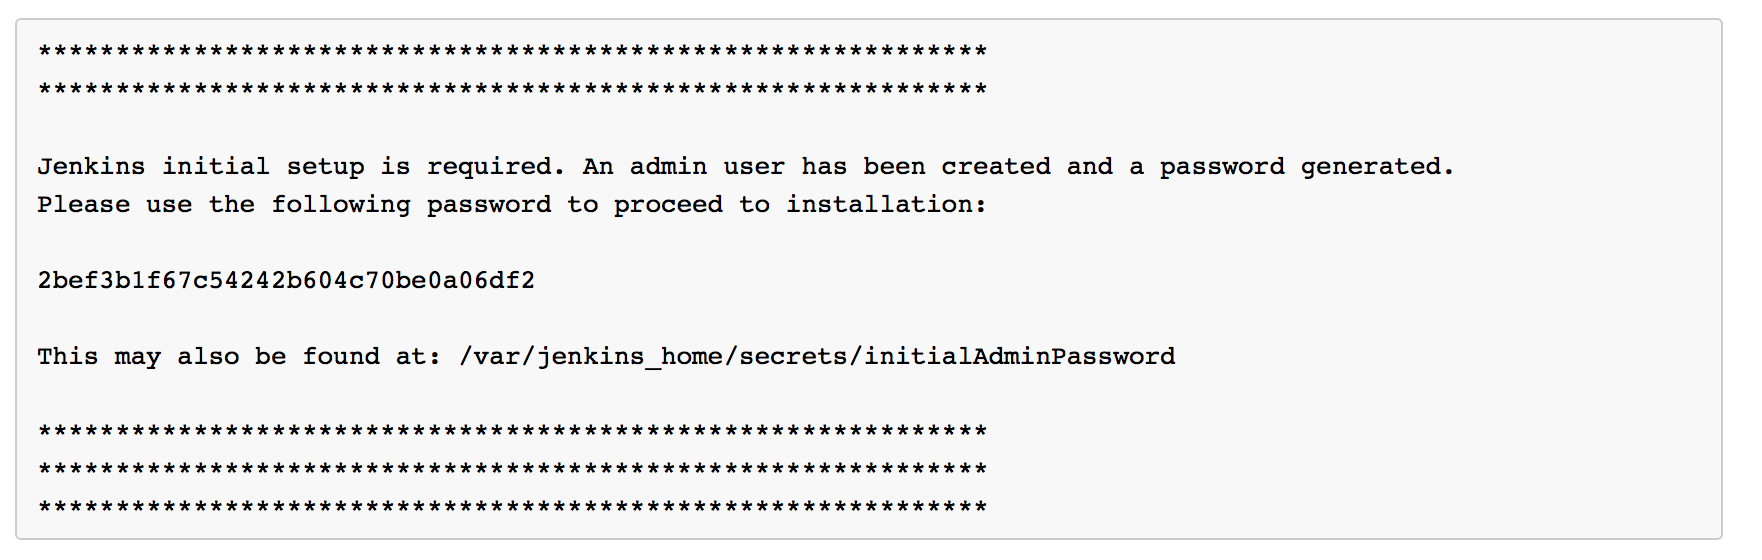
\includegraphics[width=1\textwidth]{images/09_CI/consoleOutput.png}
\caption{Konsolen Ausgabe - Jenkins}
\label{img:consoleoutput}
\end{figure}

Nachdem das initialAdminPassword ausgegeben wurde kann Jenkins unter der ServerUrl  und dem Standard Port 8080 erreicht werden. 

\begin{figure}[h]
\centering
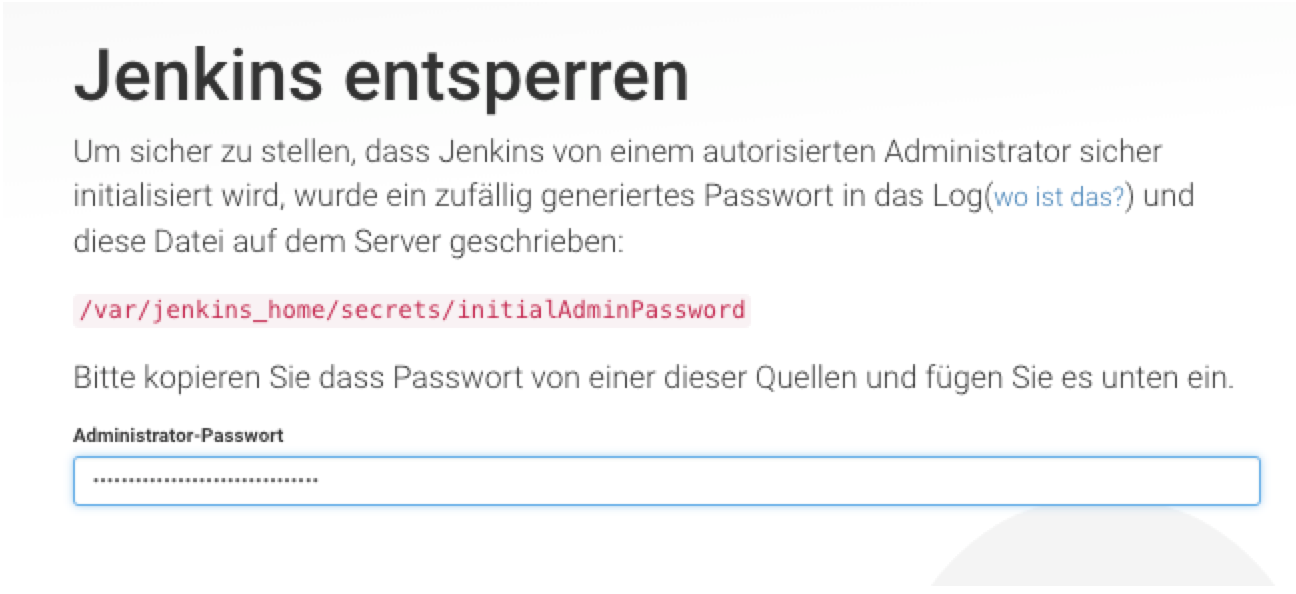
\includegraphics[width=1\textwidth]{images/09_CI/initial.png}
\caption{Anmelden - Jenkins}
\label{img:login}
\end{figure}

Wie in \ref{img:login} muss das Passwort jetzt eingegeben werden um die Installation fortzusetzen. In den nächsten Ansichten muss ein Admin User angelegt werden und die benötigten Plug-Ins für den Jenkins ausgewählt werden. Hier reichen die Standard Plug-Ins völlig aus.

Jetzt kann Jenkins verwendet werden.

\section{Jenkins CI konfigurieren}
\label{sec:jenkinsconfiguration}
Um jetzt eine JavaEE Anwendung mithilfe vom Jenkins auf einen Wildfly Application Server zu deployen müssen vorher noch die Enviroment Variablen, JDK's, Maven und der Application Server auf dem Server konfiguriert werden. Die Enviroment Variablen, JDK's und Maven werden vom Jenkins eingerichtet es muss nur in den Einstellungen die jeweilige Version konfiguriert werden. Und es muss ein Oracle Login hinterlegt werden damit sich Jenkins das Java JDK herunterladen kann. Jedoch muss aber der Wildfly manuell heruntergeladen und konfiguriert werden.

schreiben java anwendung git, pipeline konfiguration, jboss cli usw



% create further tex files for all other chapters of your document
\chapter{Summary}
Here you give a summary of your results and experiences. You can add also some design alternatives you considered, but kicked out later. Furthermore you might have some ideas how to drive the work you accomplished in further directions.



\bibliography{da_bibliography}{}
\bibliographystyle{alphaurl} % save alternatives are abbrvurl	alphaurl	plainurl	unsrturl

\listoffigures
\listoftables
\chapter*{Project Log Book}
\begin{tabular}{|l|l|l|l|}
\hline
Date & Participants & Todos & Due\\
\hline
\end{tabular}

\appendix
\chapter{Additional Information} \label{cha:additional-information}
If needed the appendix is the place where additional information concerning your thesis goes. Examples could be:
\begin{itemize}
	\item Source Code
	\item Test Protocols
	\item Project Proposal
	\item Project Plan
	\item Individual Goals
	\item \ldots
\end{itemize}
Again this has to be aligned with the supervisor.
\chapter{Individual Goals} \label{cha:individual-goals}
This is just another example to show what content could go into the appendix.
\end{document}  